\chapter{RESULTADOS}
\label{cap:resultados}

Neste capítulo são apresentados os resultados obtidos a partir dos experimentos realizados com o sistema híbrido 3DVar. Nesses experimentos, buscou-se testar os dois algoritmos de assimilação de dados EnKF e EnSRF, além dos efeitos da contribuição do conjunto de análises na determinação da matriz de covariâncias híbrida. 
A Seção \ref{sec:assim_dados_hyb_3dvar} traz os resultados relacionados a aplicação do sistema híbrido 3DVar. A verificação dos resultados é feita com base na avaliação da inovação dos conjuntos de análises e a sua contribuição na determinação das análises híbridas determinísticas. Do ponto de vista das previsões numéricas, é avaliada a habilidade das previsões de até 5 dias a partir das análises variacionais, obtidas com a aplicação da matriz de covariâncias híbrida. 

A Seção \ref{sec:estudo_caso}, contextualiza e valida a aplicação do sistema híbrido 3DVar através de um estudo de caso da Zona de Convergência do Atlântico Sul (ZCAS), em Janeiro de 2013.

\section{Assimilação de Dados Híbrida 3DVar}
\label{sec:assim_dados_hyb_3dvar}

Nesta seção são apresentados os resultados obtidos com os experimentos do sistema híbrido 3DVar utilizando a matriz estática de covariâncias dos erros de previsão do modelo BAMv0. Nos experimentos avaliados, foram verificadas as contribuições das covariâncias dos erros do conjunto de previsões, derivadas a partir dos algoritmos EnKF e EnSRF. Os resultados desta seção, estão organizados da seguinte forma: na Seção \ref{sec:inov_conj_anl}, são mostradas as estatísticas de inovação dos conjuntos de análise dos experimentos híbridos. As estatísticas de inovação apresentadas foram calculadas em relação ao erro das observações convencionais assimiladas e podem ser interpretadas como importantes indicadores do condicionamento do conjunto de análises, indicando deficiências no espalhamento do conjunto e na inflação das covariâncias. Na Seção \ref{sec:exps_obs_completo}, são apresentados os resultados obtidos com a integração por até 120 horas das análises oriundas dos experimentos. A avaliação destes resultados é feita com base na correlação de anomalias das previsões contra suas próprias análises. Por fim, na Seção \ref{sec:aval_prec}, são apresentados os resultados da avaliação das previsões de precipitação de 24 horas do modelo BAMv0, calculadas a partir das análises dos experimentos.

\subsection{Viés Ponderado dos Conjuntos de Análises}
\label{sec:inov_conj_anl}

Para uma avaliação do conjunto de análises produzido a partir da aplicação do sistema híbrido 3DVar utilizando filtro de Kalman por conjunto (EnKF/EnSRF), uma avaliação das inovações do conjunto é feita com o objetivo de se diagnosticar as deficiências no espalhamento do conjunto devido aos ajustes na inflação das covariâncias e a localização do conjunto.

Para então se verificar a forma como o espalhamento do conjunto é representado na presença dos erros das observações, as inovações do conjunto são mostradas como uma medida do quão bem representado é o espalhamento do conjunto devido as inovações trazidas pelas observações. A comparação entre as estatísticas de inovação do EnKF e EnSRF são apresentadas para três regiões diferentes: Hemisfério Norte, Trópicos e Hemisfério Sul, e somente para as observações convencionais. Para tornar o entendimento dos gráficos mais fácil, no eixo $x$ estão representadas as razões entre o desvio padrão das inovações dos \textit{priors} (i.e., o conjunto de previsões) e a raiz quadrada do espalhamento total do conjunto (Eq. \ref{eq:ens_inov}).

% \begin{equation}
% \label{eq:ens_inov}
%     IE = \frac{\sigma{(\mathbf{y}^{o}-\mathbf{H}\mathbf{x}^{b}_{k})}}{\sqrt{S+R}}
% \end{equation}

\begin{equation}
  \label{eq:ens_inov}
  VI = \frac{\delta{(\mathbf{y}^{o}-\mathbf{H}\mathbf{x}^{b}_{k})}}{\sigma{(\mathbf{y}^{o}-\mathbf{H}\mathbf{x}^{b}_{k})}}
\end{equation}

onde:

\begin{itemize}
    \item $\sigma$: é o desvio-padrão;
    \item $\mathbf{y}^{o}$: é vetor observação;
    \item $\mathbf{x}^{b}_{k}$: é o $k$-ésimo membro do conjunto de $K$ previsões;
    \item $S$: é o espalhamento do conjunto (escalar);
    \item $R$: é o erro (escalar) da observação, proveniente da matriz de covariâncias dos erros de observação ($\mathbf{R}$).
\end{itemize}

Como o desvio padrão das inovações dos \textit{priors} é normalizada pela raiz quadrada do espalhamento total, quanto menores os valores determinados, melhor é a inovação do conjunto representado. Idealmente, o desvio padrão dos \textit{priors} deve se equiparar com os valores do espalhamento total se o conjunto de análises estiver bem condicionado, i.e., com uma boa quantidade de espalhamento e valores de localização e inflação apropriadamente ajustados. No caso dos experimentos realizados, como já foi mencionado anteriormente, estes valores foram mantidos iguais entre todos os experimentos que envolveram o filtro de Kalman por conjunto.

As figuras estão apresentadas para o horário das 00Z para reduzir o tamanho das séries temporais, uma vez que não foram verificadas grandes diferenças com os demais horários. Nos painéis de cima, as linhas vermelhas (pontilhadas e contínuas) referem-se os experimentos híbridos 3DVar utilizando o EnKF, em que foi considerado 50\% de contribuição das covariâncias estáticas ($\mathbf{B}$), enquanto que as linhas azuis referem-se aos mesmos experimentos, mas denotando os casos em que 75\% de contribuição das covariâncias do conjunto de previsões foi considerado. Nos painéis de baixo, os experimentos utilizando o EnSRF estão representados pelas linhas amarela (representando a contribuição de 50\%) e verde (representando a contribuição de 75\% das covariâncias).

A Figura \ref{fig:innov_ens_00z} apresenta as estatísticas de inovação do conjunto dos experimentos híbridos 3DVar utilizando o EnKF e EnSRF para o horário das 00Z. Em geral, não foram observadas grandes diferenças com os demais horários, seja na avaliação da magnitude e da variação das amplitudes das curvas. Entretanto, pode-se afirmar que as amplitudes dos \textit{priors} (i.e., do conjunto de previsões) e dos \textit{posteriors} (i.e., do conjunto de análises) variam discretamente entre si. Isto pode ser devido as variações na disponibilidade das observações nos horários das 06 e 18Z. Para algumas variáveis, o desvio padrão dos \textit{priors} parece muito distante de concordar com o espalhamento total do conjunto. Por exemplo, a temperatura ($T$, Figuras \ref{fig:Thn00_vi}, \ref{fig:Ttr00_vi} e \ref{fig:Ths00_vi}), em todas as regiões avaliadas, saturam o desvio padrão dos \textit{priors} e se mantém com alta amplitude até o final da simulação (de 1 a 31 de Janeiro de 2013). Na região TR, $T$ (Figura \ref{fig:Ttr00_vi}) leva em torno de 20 ciclos (i.e., 5 dias) para estabilizar as estatísticas de inovação do conjunto. Uma situação semelhante ocorre na região HS (Figura \ref{fig:Ths00_vi}), também para $T$ e também na região TR para a variável $q$ (Figura \ref{fig:qtr00_vi}), em que o desvio padrão dos \textit{priors} é maior do que o espalhamento total do conjunto, além de aumentar com o tempo. Em outras palavras, isto significa que o erro das previsões tende a dominar o espalhamento, o que mostra a falta de um ajuste de inflação adequado no conjunto de previsões destas variáveis para estas regiões.

A pressão em superfície ($ps$) nas regiões HN (Figura \ref{fig:pshn00_vi}), mostra que o desvio padrão dos \textit{priors} tende a crescer com o tempo, mas que isso é compensado pelo espalhamento do conjunto indicando que o conjunto de previsões tenta se ajustar as observações ainda com algum espalhamento. Uma situação diferente nas regiões TR e HS onde o desvio padrão dos \textit{priors} para $ps$ (Figuras \ref{fig:pstr00_vi}, \ref{fig:pshs00_vi}) também é maior do que o espalhamento do conjunto, mas negativo. O sinal negativo do desvio padrão dos \textit{priors}, neste caso, indica que o desvio padrão da inovação do conjunto (i.e., $\sigma{(\mathbf{y}^{o}-\mathbf{H}\mathbf{x}_{k}^{e})}$) é negativo, como se as previsões tentassem corrigir as observações.

Diferenças entre a quantidade relativa de contribuição do conjunto (i.e., as diferenças entre as contribuições de 50\% e 75\%, independente do tipo de filtro de Kalman utilizado), parecem ser mais ou menos sensíveis para algumas variáveis. Para $ps$ na região $TR$ e $HS$ (Figuras \ref{fig:pstr00_vi}, \ref{fig:pshs00_vi}), está claro que com 50\% de contribuição das covariâncias fluxo-dependentes do EnKF as covariâncias estáticas, é um valor razoável se comparado com os 75\% e contribuição do EnSRF, independente do horário sinótico (se 00 ou 12Z). Isto pode ser devido ao fato de a perturbação das observações serem realizadas no algoritmo do EnKF, quando o conjunto de previsões tem um papel mais importante na determinação dos desvios padrão nas estatísticas de inovação.

Do ponto de vista das diferenças entre os experimentos com o EnKF e o EnSRF, em geral, os resultados mostram que utilizando o sistema híbrido com o EnSRF, as diferenças entre os \textit{priors} e \textit{posteriors} são maiores do que o que foi encontrado com o EnKF. As Figuras \ref{fig:Thn00_vi}, \ref{fig:Ttr00_vi} e \ref{fig:Ths00_vi} com as estatísticas de inovação do conjunto para a variável $T$ nas regiões HN, TR e HS (independentemente da contribuição relativa das covariâncias do conjunto), mostram que estas diferenças são mais evidentes no HN, em que $T$ é mais próxima de zero com o EnSRF do que com o EnKF. Este é um resultado desejável, uma vez que o desvio padrão dos da inovação dos \textit{priors} se equipara com o espalhamento total do conjunto.

O desvio padrão do vento horizontal ($uv$) sobre a região HN (Figura \ref{fig:uvhn00_vi}), é muito próximo do espalhamento total do conjunto, indicando que o ajuste do conjunto de previsões as observações foi bom e que a quantidade de espalhamento parece ser razoável. Na região TR (Figura \ref{fig:uvtr00_vi}), entretanto, foi encontrado o contrário, em que durante todo o período de simulações, o desvio-padrão dos \textit{priors} dominou a relação com o espalhamento total do conjunto. Na região HS (Figura \ref{fig:uvhs00_vi}), ocorreu uma situação semelhante ao que foi encontrado na região HN em que a amplitude do sinal da inovação do conjunto aumenta, indicando, possivelmente, deficiências na inflação no conjunto devido ao reduzido número de observações na região.

\begin{figure}[H]
    \vspace{-8mm}
    \caption{Estatísticas de inovação dos conjuntos de análises dos experimentos, válido para as 00Z.}
    \begin{center}
        \subfigure[$uv$, HN]{
            \label{fig:uvhn00_vi}
            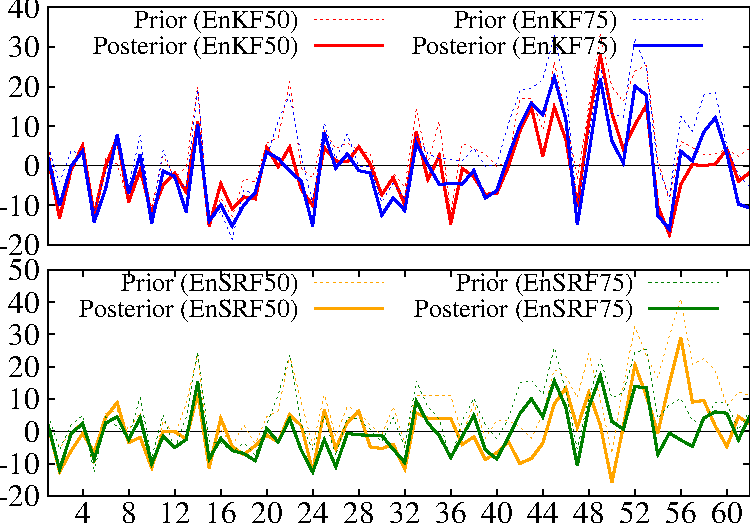
\includegraphics[width=0.3095\textwidth]{./figs/cap5/estat_inov_ens/00Z/baseline_innov_stats_priors_NH_uv-00Z-novas-legenda-crop.pdf}
        }
        \subfigure[$uv$, TR]{
          \label{fig:uvtr00_vi}
          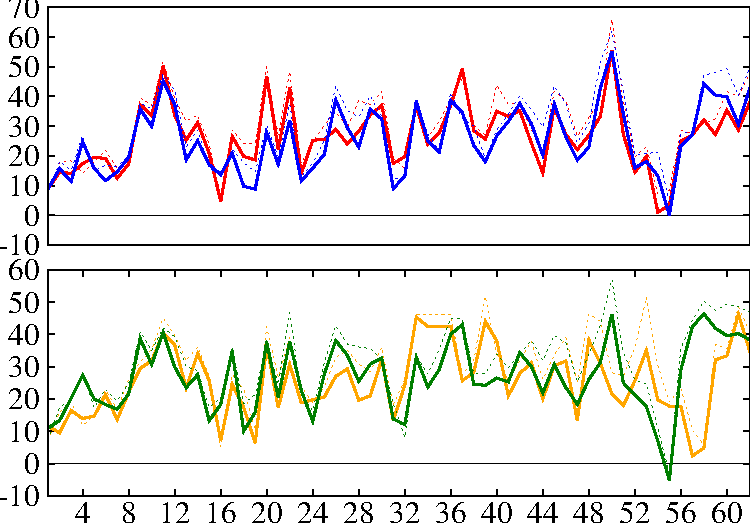
\includegraphics[width=0.3095\textwidth]{./figs/cap5/estat_inov_ens/00Z/baseline_innov_stats_priors_TR_uv-00Z-novas-crop.pdf}
        }
        \subfigure[$uv$, HS]{
          \label{fig:uvhs00_vi}
          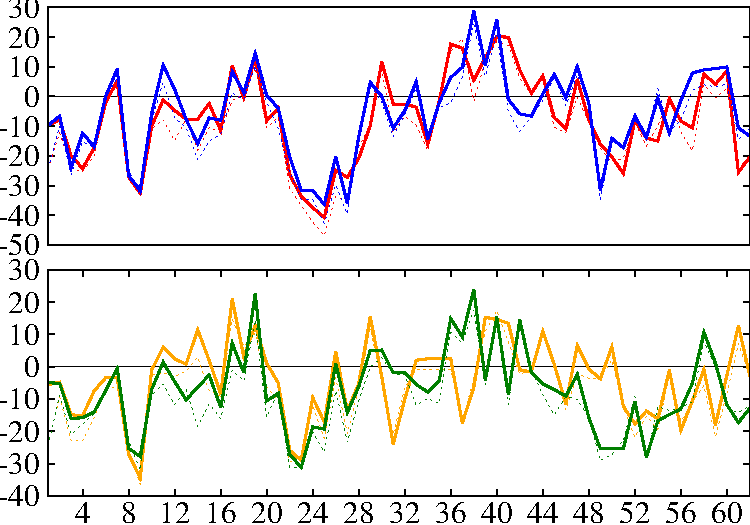
\includegraphics[width=0.3095\textwidth]{./figs/cap5/estat_inov_ens/00Z/baseline_innov_stats_priors_SH_uv-00Z-novas-crop.pdf}
        }\\     
        \subfigure[$T$, HN]{
            \label{fig:Thn00_vi}
            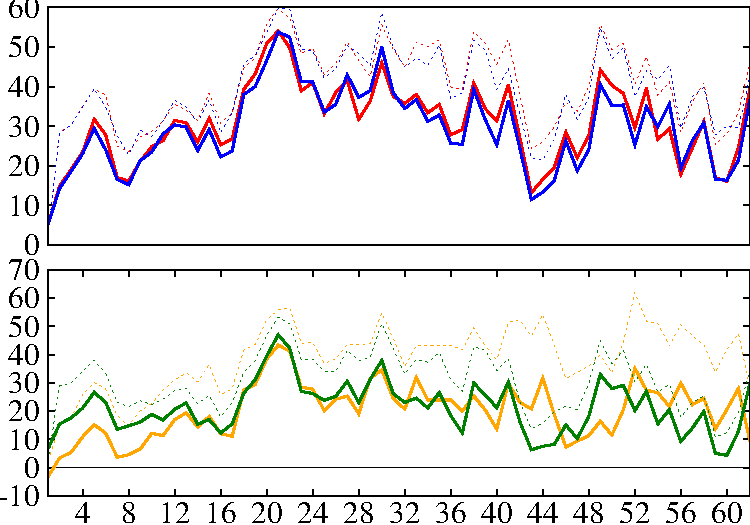
\includegraphics[width=0.3095\textwidth]{./figs/cap5/estat_inov_ens/00Z/baseline_innov_stats_priors_NH_t-00Z-novas-crop.pdf}
        }
        \subfigure[$T$, TR]{
          \label{fig:Ttr00_vi}
          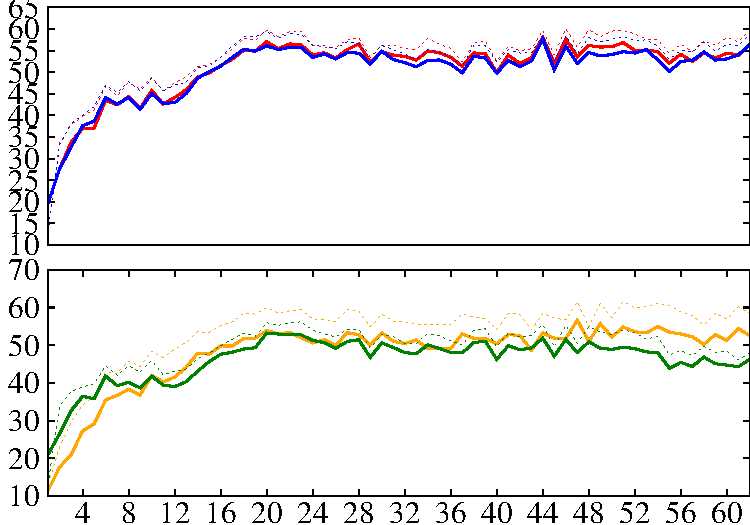
\includegraphics[width=0.3095\textwidth]{./figs/cap5/estat_inov_ens/00Z/baseline_innov_stats_priors_TR_t-00Z-novas-crop.pdf}
        }
        \subfigure[$T$, HS]{
            \label{fig:Ths00_vi}
            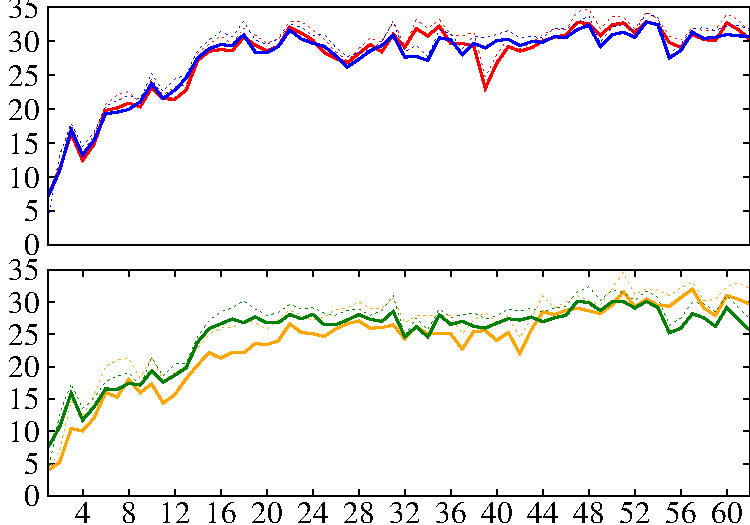
\includegraphics[width=0.3095\textwidth]{./figs/cap5/estat_inov_ens/00Z/baseline_innov_stats_priors_SH_t-00Z-novas-crop.pdf}
        }\\
        \subfigure[$q$, HN]{
            \label{fig:qhn00_vi}
            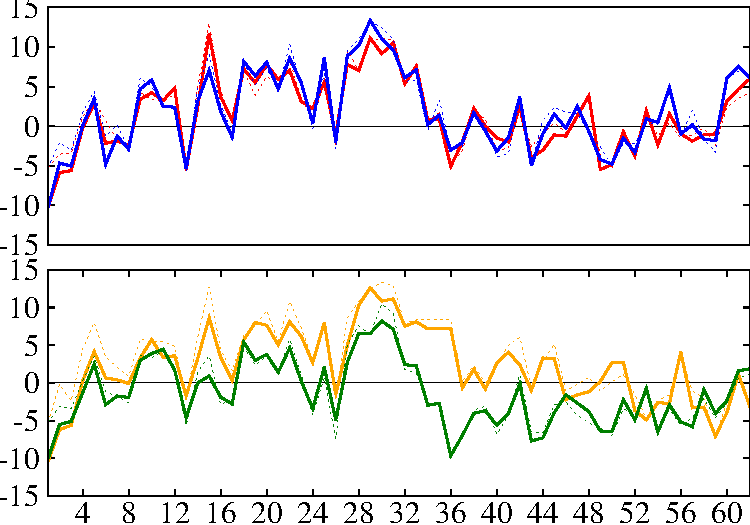
\includegraphics[width=0.3095\textwidth]{./figs/cap5/estat_inov_ens/00Z/baseline_innov_stats_priors_NH_q-00Z-novas-crop.pdf}
        }
        \subfigure[$q$, TR]{
          \label{fig:qtr00_vi}
          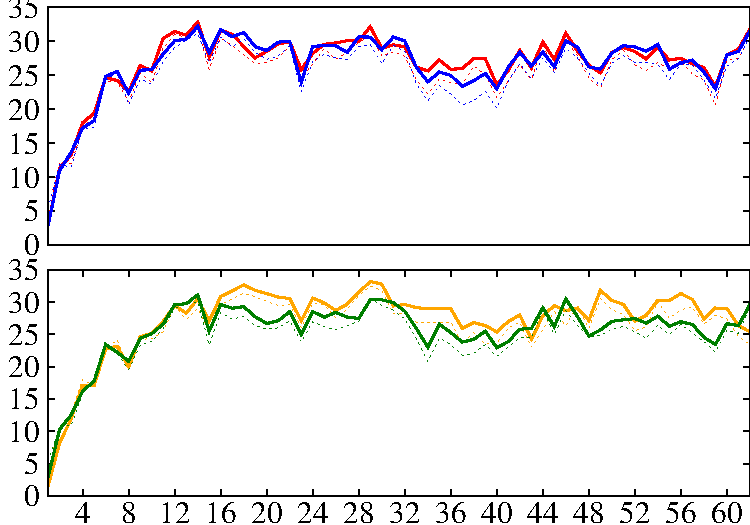
\includegraphics[width=0.3095\textwidth]{./figs/cap5/estat_inov_ens/00Z/baseline_innov_stats_priors_TR_q-00Z-novas-crop.pdf}
        }
        \subfigure[$q$, HS]{
            \label{fig:qhs00_vi}
            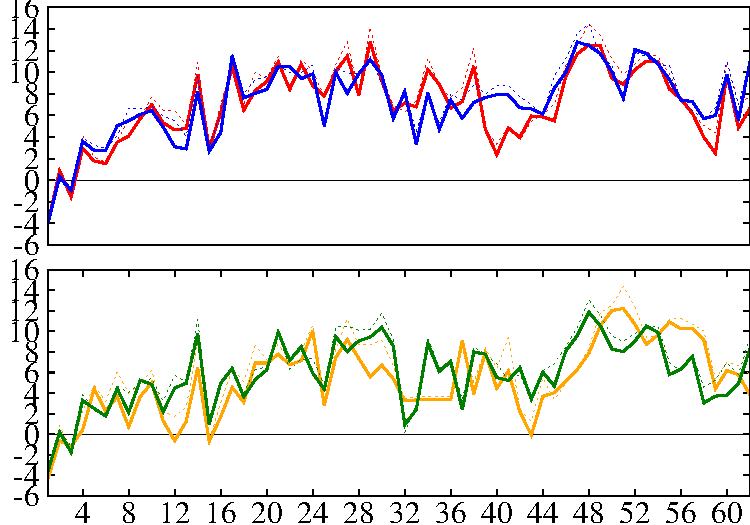
\includegraphics[width=0.3095\textwidth]{./figs/cap5/estat_inov_ens/00Z/baseline_innov_stats_priors_SH_q-00Z-novas-crop.pdf}
        }\\
        \subfigure[$gps$, HN]{
            \label{fig:gpshn00_vi}
            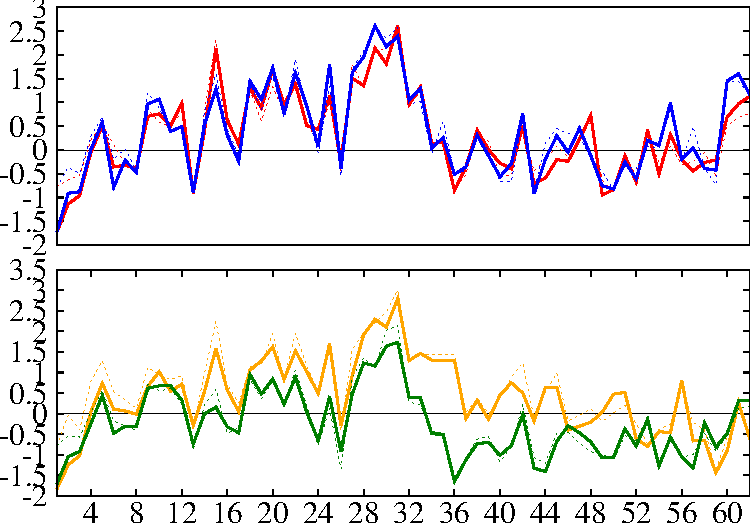
\includegraphics[width=0.3095\textwidth]{./figs/cap5/estat_inov_ens/00Z/baseline_innov_stats_priors_NH_gps-00Z-novas-crop.pdf}
        }
        \subfigure[$gps$, TR]{
          \label{fig:gpstr00_vi}
          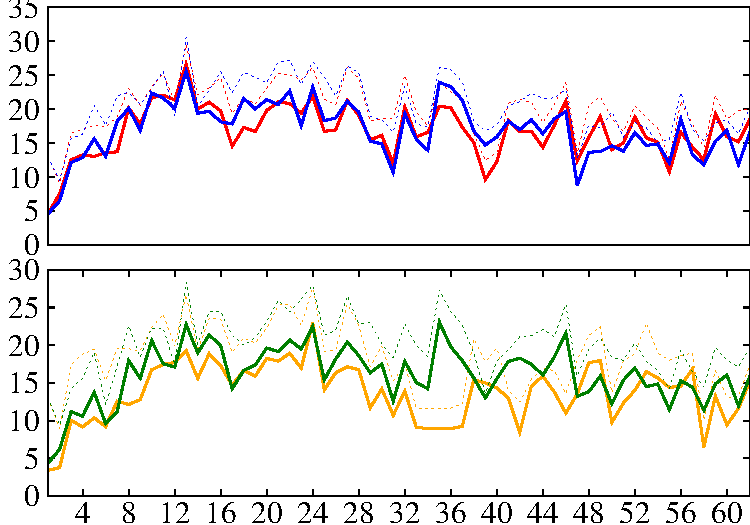
\includegraphics[width=0.3095\textwidth]{./figs/cap5/estat_inov_ens/00Z/baseline_innov_stats_priors_TR_gps-00Z-novas-crop.pdf}
        }
        \subfigure[$gps$, HS]{
          \label{fig:gpshs00_vi}
          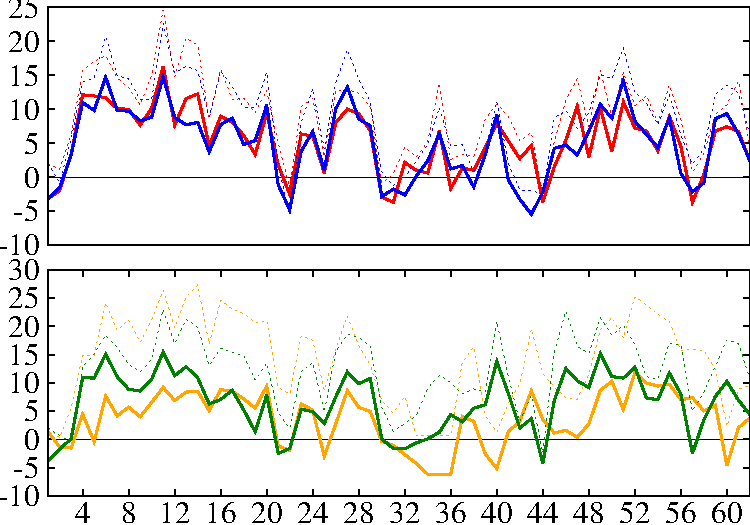
\includegraphics[width=0.3095\textwidth]{./figs/cap5/estat_inov_ens/00Z/baseline_innov_stats_priors_SH_gps-00Z-novas-crop.pdf}
        }\\
        \subfigure[$ps$, HN]{
            \label{fig:pshn00_vi}
            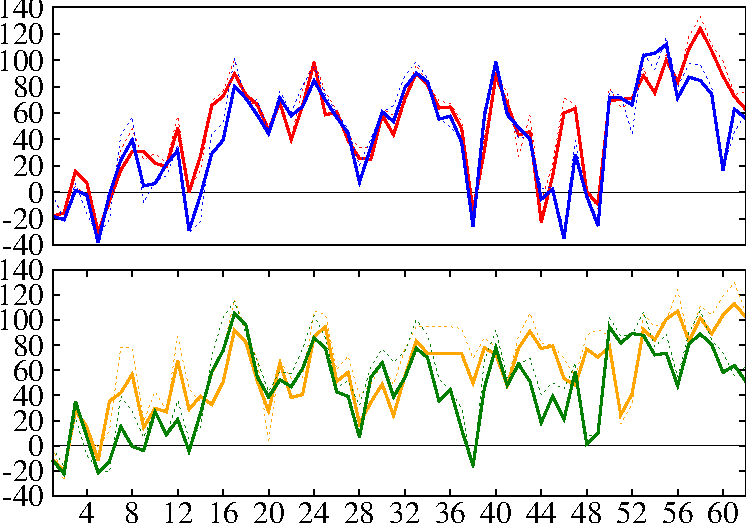
\includegraphics[width=0.3095\textwidth]{./figs/cap5/estat_inov_ens/00Z/baseline_innov_stats_priors_NH_ps-00Z-novas-crop.pdf}
        }
        \subfigure[$ps$, TR]{
          \label{fig:pstr00_vi}
          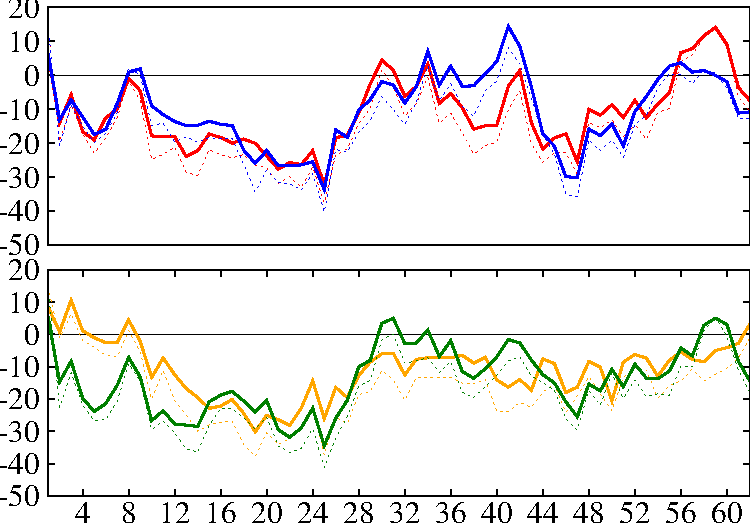
\includegraphics[width=0.3095\textwidth]{./figs/cap5/estat_inov_ens/00Z/baseline_innov_stats_priors_TR_ps-00Z-novas-crop.pdf}
        }     
        \subfigure[$ps$, HS]{
          \label{fig:pshs00_vi}
          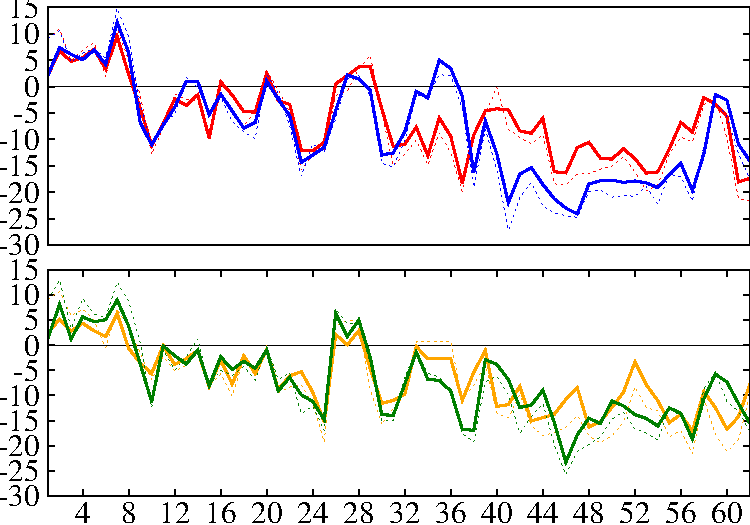
\includegraphics[width=0.3095\textwidth]{./figs/cap5/estat_inov_ens/00Z/baseline_innov_stats_priors_SH_ps-00Z-novas-crop.pdf}
        }        
    \end{center}
    \vspace{2mm}
    \legenda{Em vermelho (azul) estão representadas as inovações com 50\% (75\%) de contribuição das covariâncias do EnKF. Em laranja (verde), as inovações com 50\% (75\%) de contribuição do EnSRF. As linhas pontilhadas representam os \textit{priors} e as linhas sólidas, os \textit{posteriors}. A esquerda, os resultados para o Hemisfério Norte (HN); meio para os Trópicos (TR) e a direita, Hemisfério Sul (HS).}
  \label{fig:innov_ens_00z_vi}
  \FONTE{Produção do autor.}
\end{figure}

\subsection{Inovação dos Conjuntos de Análises}
\label{sec:inova_ens}

\begin{equation}
    IC = \frac{\sigma{(\mathbf{y}^{o}-\mathbf{H}\mathbf{x}^{b}_{k})}}{\sqrt{S+R}}
\end{equation}

\newpage

\begin{figure}[H]
    \vspace{-8mm}
    \caption{Estatísticas de inovação dos conjuntos de análises dos experimentos, válido para as 00Z.}
    \begin{center}

        \subfigure[$uv$, HN]{
            \label{fig:uvhn00_ic}
            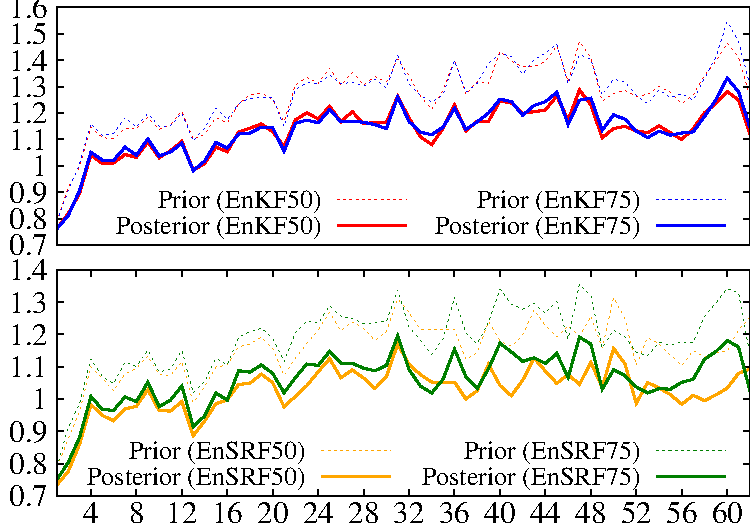
\includegraphics[width=0.3095\textwidth]{./figs/cap5/estat_inov_ens_novas/baseline_innov_stats_priors2_NH_uv-00Z-novas-legenda.pdf}
        }
        \subfigure[$uv$, TR]{
          \label{fig:uvtr00_ic}
          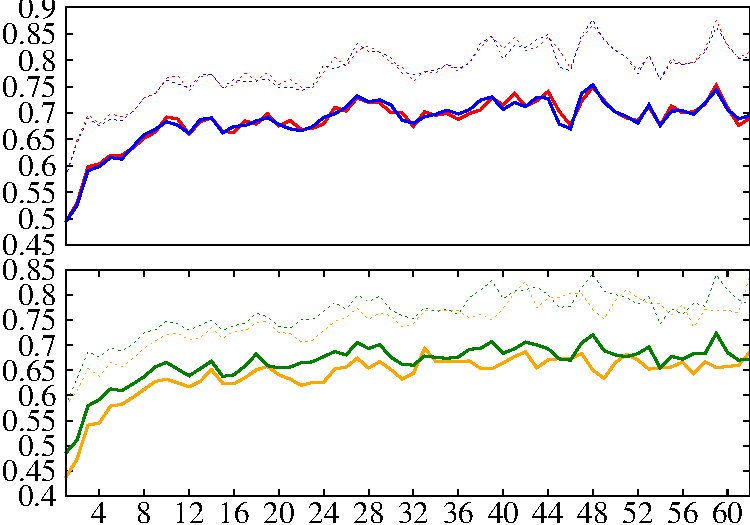
\includegraphics[width=0.3095\textwidth]{./figs/cap5/estat_inov_ens_novas/baseline_innov_stats_priors2_TR_uv-00Z-novas.pdf}
        }
        \subfigure[$uv$, HS]{
          \label{fig:uvhs00_ic}
          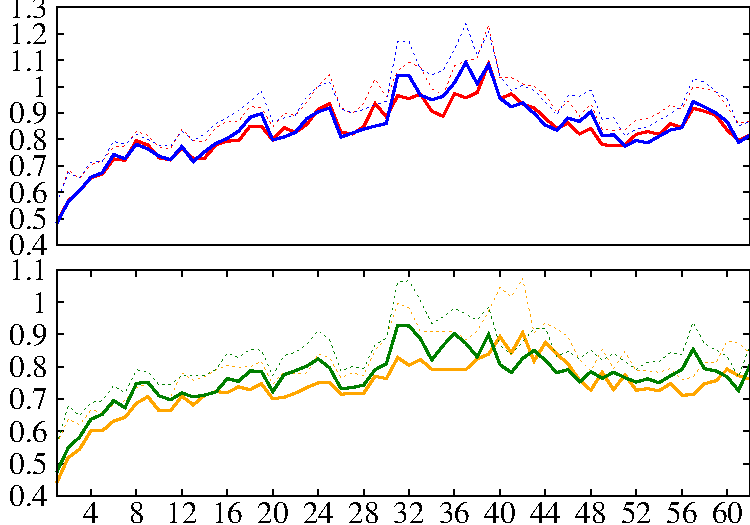
\includegraphics[width=0.3095\textwidth]{./figs/cap5/estat_inov_ens_novas/baseline_innov_stats_priors2_SH_uv-00Z-novas.pdf}
        }\\     
        \subfigure[$T$, HN]{
            \label{fig:Thn00_ic}
            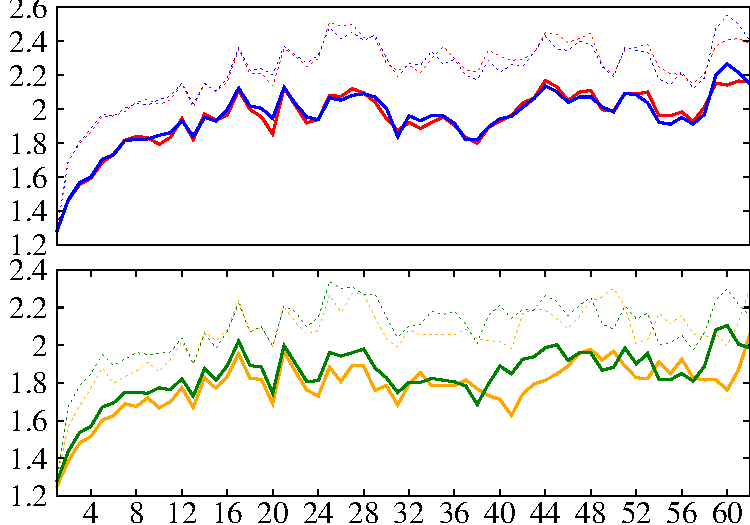
\includegraphics[width=0.3095\textwidth]{./figs/cap5/estat_inov_ens_novas/baseline_innov_stats_priors2_NH_t-00Z-novas.pdf}
        }
        \subfigure[$T$, TR]{
          \label{fig:Ttr00_ic}
          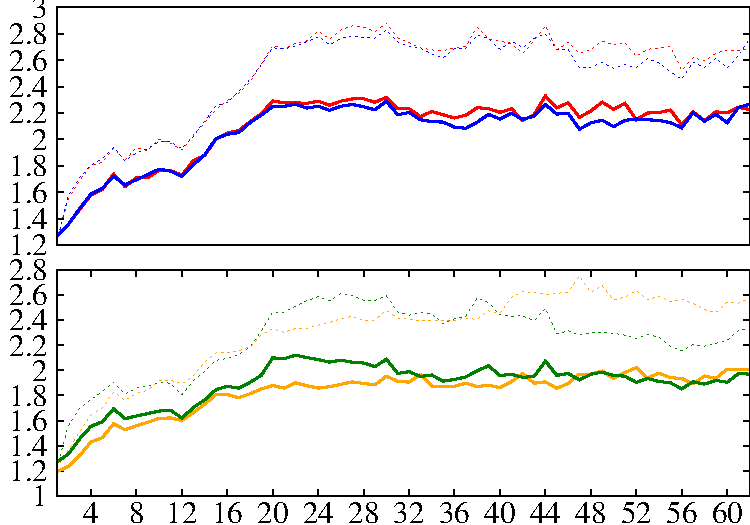
\includegraphics[width=0.3095\textwidth]{./figs/cap5/estat_inov_ens_novas/baseline_innov_stats_priors2_TR_t-00Z-novas.pdf}
        }
        \subfigure[$T$, HS]{
            \label{fig:Ths00_ic}
            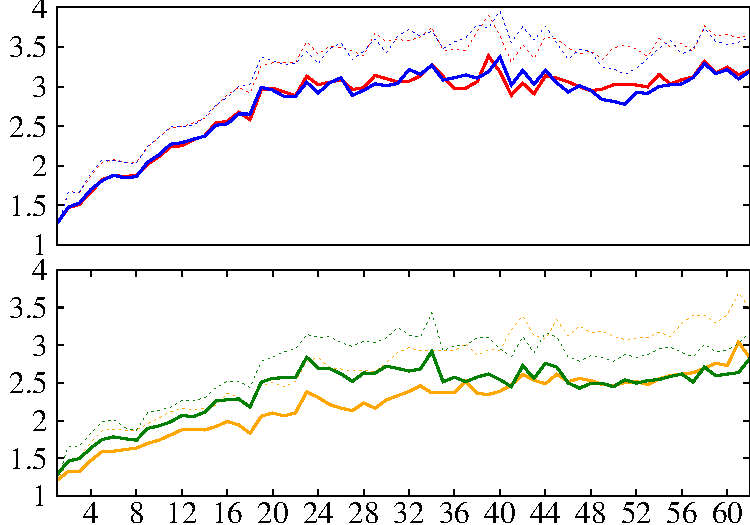
\includegraphics[width=0.3095\textwidth]{./figs/cap5/estat_inov_ens_novas/baseline_innov_stats_priors2_SH_t-00Z-novas.pdf}
        }\\
        \subfigure[$q$, HN]{
            \label{fig:qhn00_ic}
            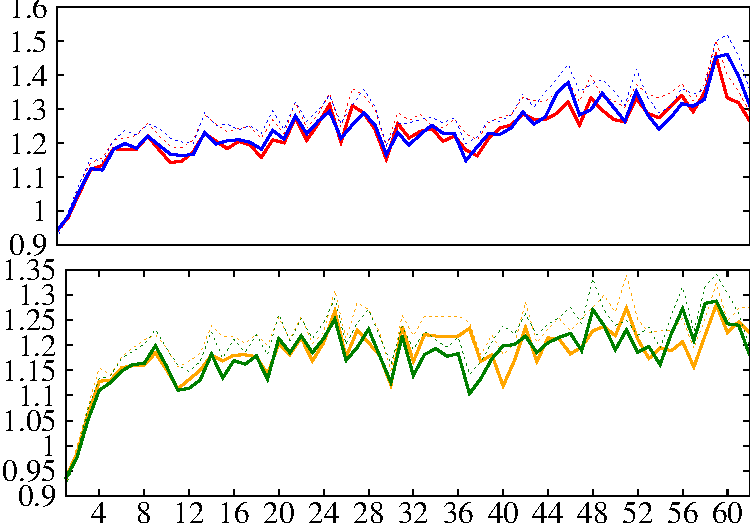
\includegraphics[width=0.3095\textwidth]{./figs/cap5/estat_inov_ens_novas/baseline_innov_stats_priors2_NH_q-00Z-novas.pdf}
        }
        \subfigure[$q$, TR]{
          \label{fig:qtr00_ic}
          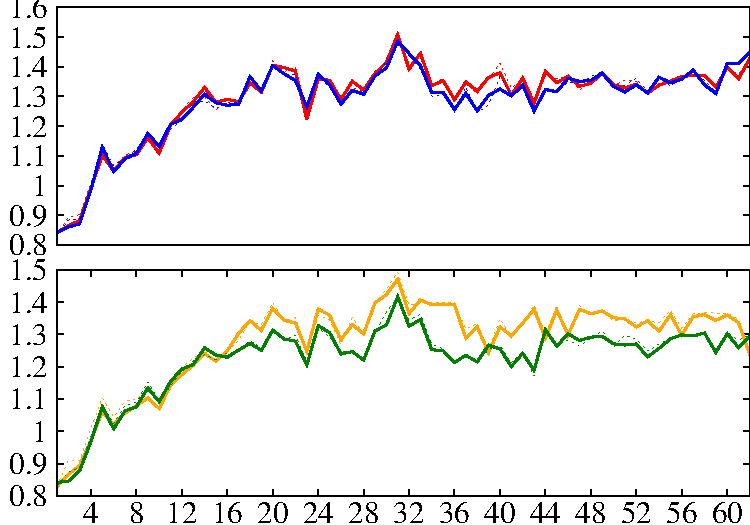
\includegraphics[width=0.3095\textwidth]{./figs/cap5/estat_inov_ens_novas/baseline_innov_stats_priors2_TR_q-00Z-novas.pdf}
        }
        \subfigure[$q$, HS]{
            \label{fig:qhs00_ic}
            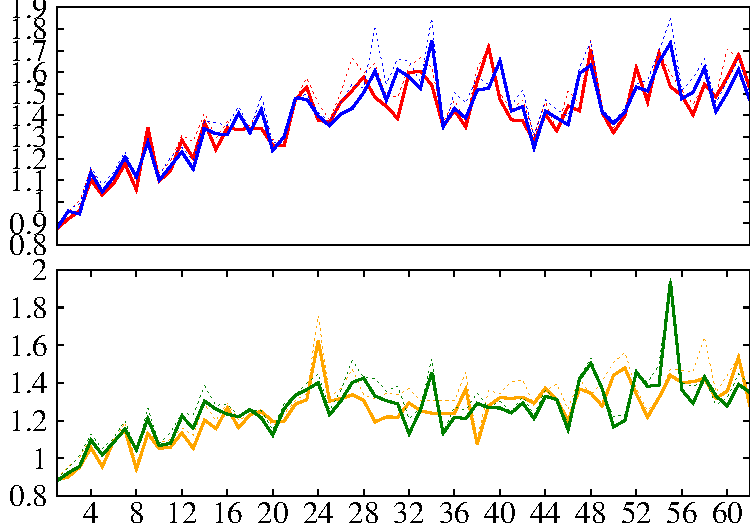
\includegraphics[width=0.3095\textwidth]{./figs/cap5/estat_inov_ens_novas/baseline_innov_stats_priors2_SH_q-00Z-novas.pdf}
        }\\
        \subfigure[$gps$, HN]{
            \label{fig:gpshn00_ic}
            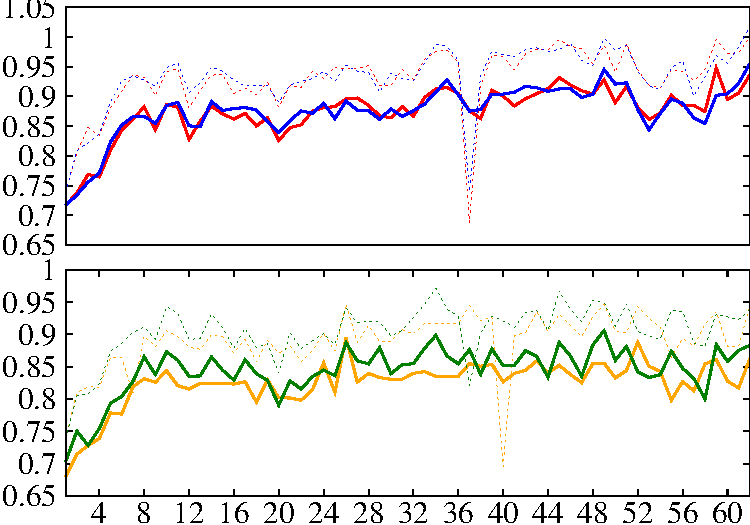
\includegraphics[width=0.3095\textwidth]{./figs/cap5/estat_inov_ens_novas/baseline_innov_stats_priors2_NH_gps-00Z-novas.pdf}
        }
        \subfigure[$gps$, TR]{
          \label{fig:gpstr00_ic}
          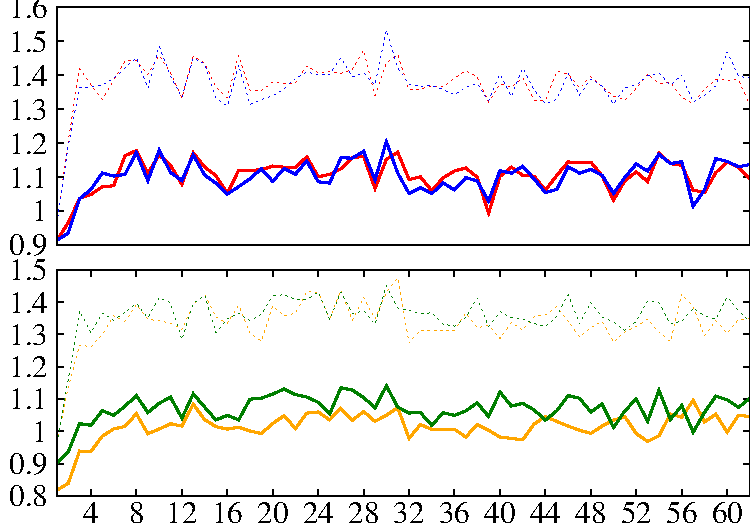
\includegraphics[width=0.3095\textwidth]{./figs/cap5/estat_inov_ens_novas/baseline_innov_stats_priors2_TR_gps-00Z-novas.pdf}
        }
        \subfigure[$gps$, HS]{
          \label{fig:gpshs00_ic}
          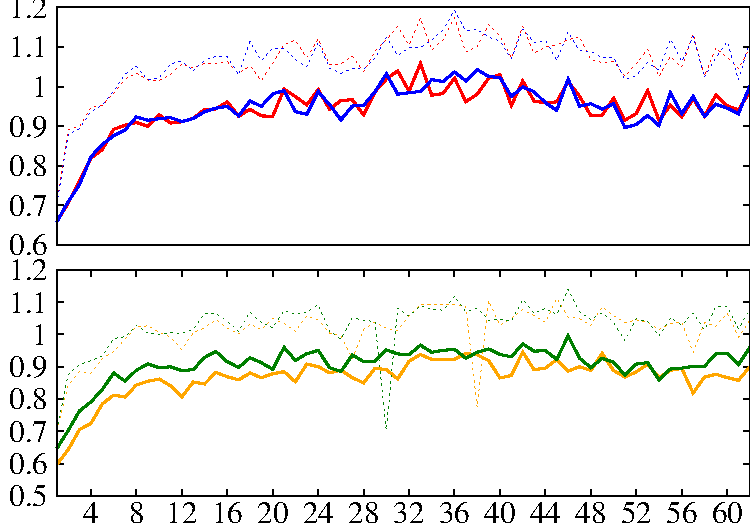
\includegraphics[width=0.3095\textwidth]{./figs/cap5/estat_inov_ens_novas/baseline_innov_stats_priors2_SH_gps-00Z-novas.pdf}
        }\\
        \subfigure[$ps$, HN]{
            \label{fig:pshn00_ic}
            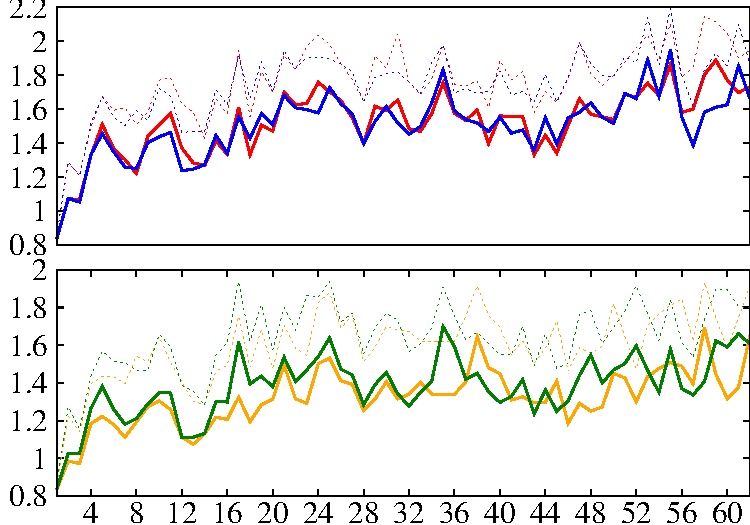
\includegraphics[width=0.3095\textwidth]{./figs/cap5/estat_inov_ens_novas/baseline_innov_stats_priors2_NH_ps-00Z-novas.pdf}
        }
        \subfigure[$ps$, TR]{
          \label{fig:pstr00_ic}
          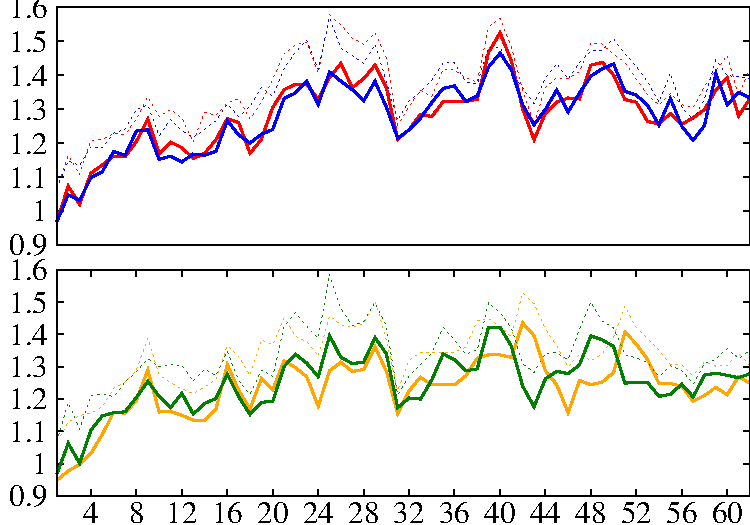
\includegraphics[width=0.3095\textwidth]{./figs/cap5/estat_inov_ens_novas/baseline_innov_stats_priors2_TR_ps-00Z-novas.pdf}
        }     
        \subfigure[$ps$, HS]{
          \label{fig:pshs00_ic}
          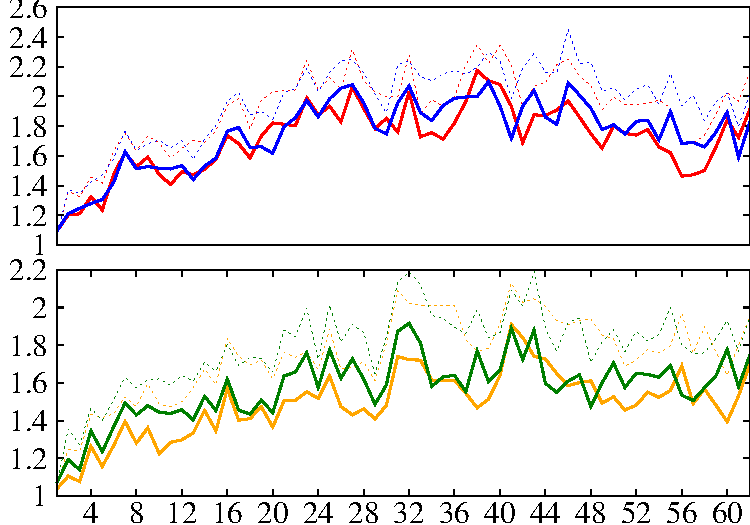
\includegraphics[width=0.3095\textwidth]{./figs/cap5/estat_inov_ens_novas/baseline_innov_stats_priors2_SH_ps-00Z-novas.pdf}
        }        
    \end{center}
    \vspace{2mm}
    \legenda{Em vermelho (azul) estão representadas as inovações com 50\% (75\%) de contribuição das covariâncias do EnKF. Em laranja (verde), as inovações com 50\% (75\%) de contribuição do EnSRF. As linhas pontilhadas representam os \textit{priors} e as linhas sólidas, os \textit{posteriors}. A esquerda, os resultados para o Hemisfério Norte (HN); meio para os Trópicos (TR) e a direita, Hemisfério Sul (HS).}
  \label{fig:innov_ens_00z_ic}
  \FONTE{Produção do autor.}
\end{figure}

\subsection{Habilidade das Previsões até 120 horas}
\label{sec:exps_obs_completo}

Os resultados apresentados a seguir referem-se a habilidade da previsão do modelo BAMv0 para até 120 horas (5 dias) a partir das análises dos experimentos REF, 3DVar puro e híbridos 3DVar (conforme discutido na Seção \ref{sec:exps}). Em todos os experimentos, foram utilizadas as mesmas configurações do modelo BAMv0 na resolução TQ0062L028 e, nos experimentos com ciclos de assimilação de dados, a versão da matriz de covariâncias estática é a mesma. 

A habilidade de previsão do modelo BAMv0 para até 5 dias foi avaliada em termos da Correlação de Anomalia (CA). Como os desenvolvimentos do CPTEC tem foco sobre as regiões Tropical e América do Sul, a habilidade de previsão do modelo de circulação geral do CPTEC foi feita para as seguintes regiões: Globo (GL), Hemisfério Norte (HN), Trópicos (TR), Hemisfério Sul (HS) e América do Sul (AS).Para se verificar o quão diferentes são os experimentos entre si, um teste de significância t-Student foi aplicado para cada caso com um nível de confiança de 95\%. Para cada figura de correlação de anomalia (painéis de cima), tem-se portanto, uma figura em anexo (painéis de baixo) mostrando os resultados do teste. No teste de significância, há uma curva correspondente a cada experimento (exceto o experimento de referência, REF). Quando as curvas cruzam suas respectivas caixas (cada caixa e curva possui uma cor distinta), há a indicação de que a diferença entre o experimento (e.g., experimento EnKF50) e a referência (e.g., experimento REF) não é significativa, e que, portanto, o teste da hipótese nula falha. Nesta avaliação, a hipótese nula estabelece que a média do experimento (híbridos 3DVar ou 3DVar puro) verificado é estatisticamente indistinguível da média do experimento de referência.

Na Figura \ref{fig:skill_nh_tr_sh} são apresentados os resultados da CA para as previsões de até 5 dias com o teste t-Student dos experimentos para as regiões HN, TR e HS. A Figura \ref{fig:skill_gl_sa} apresenta os resultados para as regiões GL e AS. As variáveis avaliadas são a pressão em superfície $psnm$, a umidade específica em 925 hPa ($q925$), a temperatura do ar em 850 hPa ($T850$), a componente zonal do vento em 250 hPa ($u250$) e a altura geopotencial em 500 hPa ($z500$). Em geral, os experimento EnKF75 e EnSRF50 indicam as análises que produziram as previsões com maiores valores de correlação, para todas as regiões e variáveis avaliadas. A $psnm$ sobre o HN (Figura \ref{fig:psnmhn0012}) não apresenta diferenças distinguíveis entre os experimentos EnKF75 e EnSRF50, para as primeiras 24 horas de previsão. Este resultado indica que na análise da pressão em superfície do sistema 3DVar, pouco da contribuição dos 50\% das covariâncias do conjunto de previsões foi utilizada ou que realmente modificou as covariâncias estáticas. Isto pode ser devido ao fato de que as observações utilizadas pelo EnSRF não foram perturbadas, o que por sua vez pode não ter sido benéfico para a análise híbrida deste sistema.

Na região TR, - uma região particularmente de difícil previsão - as previsões de $psnm$, $q925$ e $T850$ (Figuras \ref{fig:psnmtr0012}, \ref{fig:q925tr0012} e \ref{fig:T850tr0012}), para ambos os experimentos EnKF75 e EnSRF50, mostraram-se com boa performance em relação aos experimentos REF e 3DVar. As melhorias em relação do experimento REF para a $psnm$ (Figura \ref{fig:psnmtr0012}), são de quase 24 horas (considerando o limite de 80\% de CA). A Figura \ref{fig:q925tr0012} mostra as melhorias de $q925$ apresentadas pelo experimento EnSRF75 em relação ao experimento 3DVar com praticamente 4 dias de antecedência (considerando-se 85\% de CA). Uma melhoria semelhante foi também encontrada para a $T850$ (Figura \ref{fig:T850tr0012}), em comparação com o experimento 3DVar, em que o experimento EnSRF75 permanece com 80\% de CA na previsão de 72 horas, enquanto o experimento 3DVar limita sua habilidade de previsão em apenas 36 horas, considerando-se o mesmo nível de habilidade de previsão que o experimento EnSRF75. Nas Figuras \ref{fig:psnmtr0012}, \ref{fig:T850tr0012} e \ref{fig:z500tr0012} pode-se observar o tempo que o modelo BAMv0 leva para se estabilizar quando iniciado com as análises do NCEP (experimento REF). No entanto, este efeito não foi observado para todas as variáveis. Na Figura \ref{fig:T850hn0012}, por exemplo, indica que há não diferenças práticas entre os experimentos com CA semelhante. O teste t-Student, entretanto, revela que o experimento 3DVar não falha o teste da hipótese nula para as 120 horas de previsão, enquanto que o resto dos experimentos falham no teste em até 36 horas (experimentos EnKF50 e ENSRF50) e 72 horas (EnKF75 e EnSRF75). Por outro lado, os experimentos com 75\% de contribuição das covariâncias do conjunto, são estatisticamente diferentes do experimento REF até 72 horas de previsão.

\begin{figure}[H]
    \vspace{-4mm}
    \caption{Correlação de Anomalia com teste de significância t-Student (95\%) das previsões para até 120 horas para os horários das 00 e 12Z, sobre as regiões Hemisfério Norte (HN), Trópicos (TR) e Hemisfério Sul (HS).}
    \begin{center}
        \subfigure[$psnm$ - 00 e 12Z, HN]{
            \label{fig:psnmhn0012}
            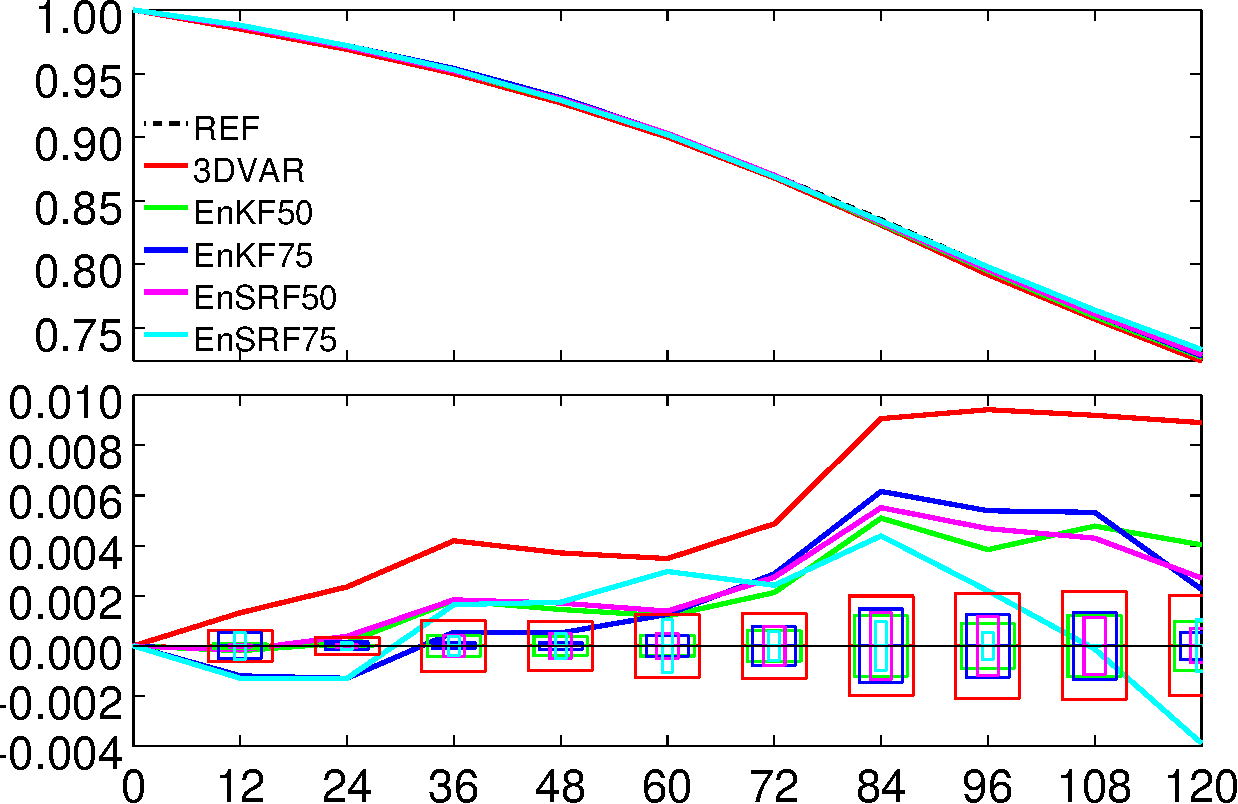
\includegraphics[width=0.3095\textwidth]{./figs/cap5/skill_prevs120h/0012z/ACOR_psnm000_hnorte-0012z-legenda-crop.pdf}
        }
        \subfigure[$psnm$ - 00 e 12Z, TR]{
          \label{fig:psnmtr0012}
          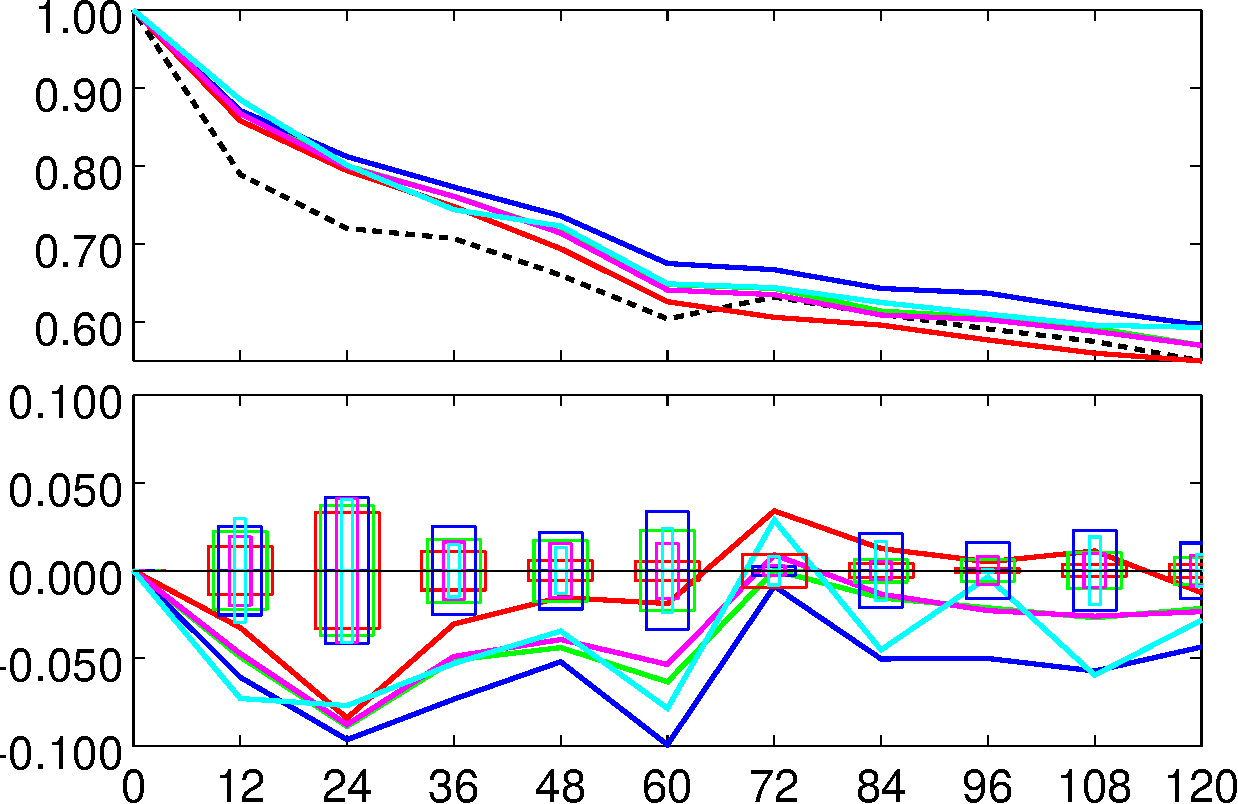
\includegraphics[width=0.3095\textwidth]{./figs/cap5/skill_prevs120h/0012z/ACOR_psnm000_tropic-0012z-crop.pdf}
        }
        \subfigure[$psnm$ - 00 e 12Z, HS]{
          \label{fig:psnmhs0012}
          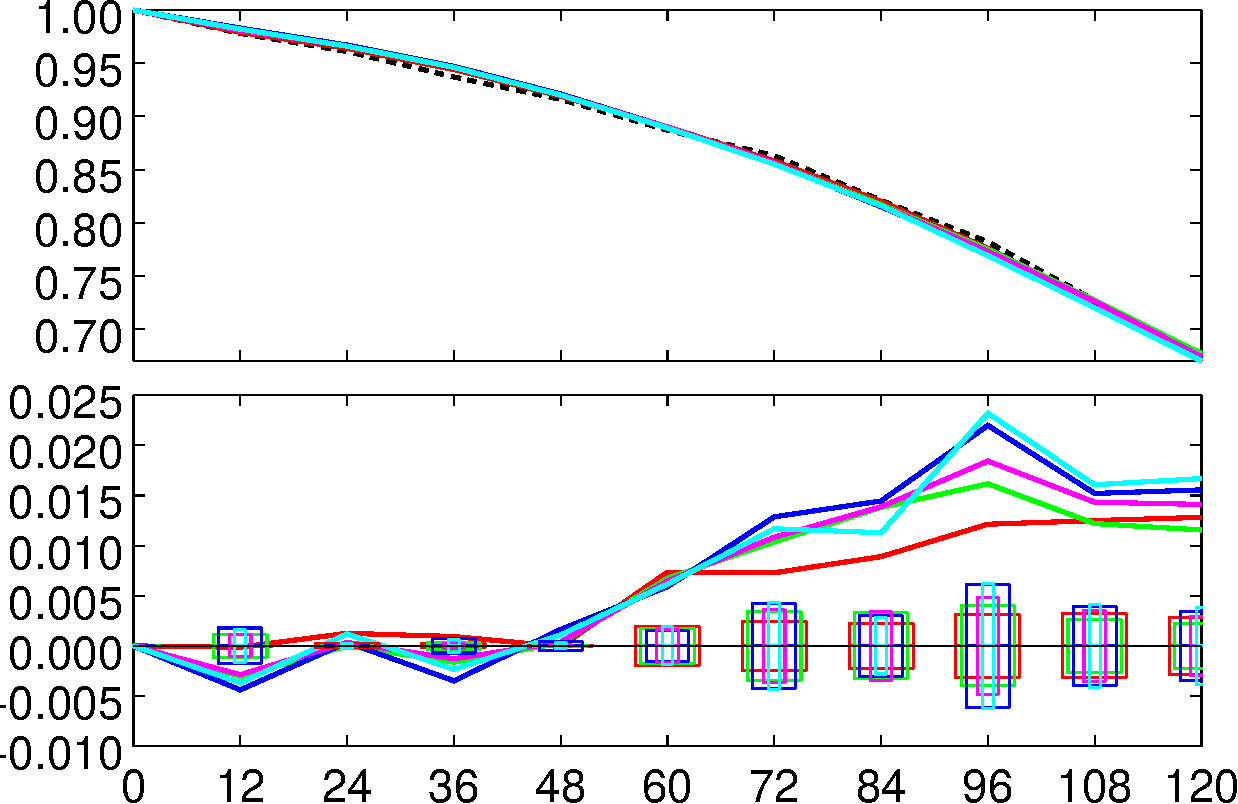
\includegraphics[width=0.3095\textwidth]{./figs/cap5/skill_prevs120h/0012z/ACOR_psnm000_hemsul-0012z-crop.pdf}
        }\\     
        \subfigure[$q$ 925 hPa - 00 e 12Z, HN]{
            \label{fig:q925hn0012}
            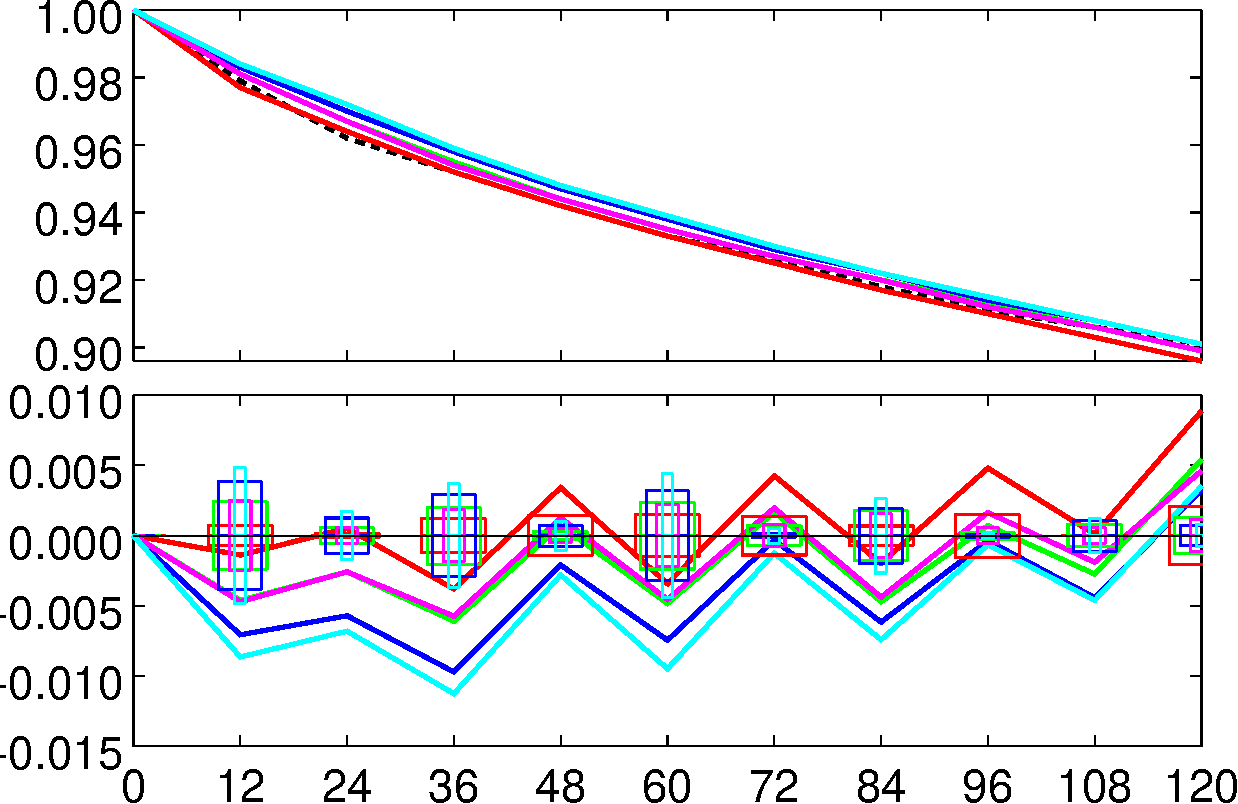
\includegraphics[width=0.3095\textwidth]{./figs/cap5/skill_prevs120h/0012z/ACOR_umes925_hnorte-0012z-crop.pdf}
        }
        \subfigure[$q$ 925 hPa - 00 e 12Z, TR]{
          \label{fig:q925tr0012}
          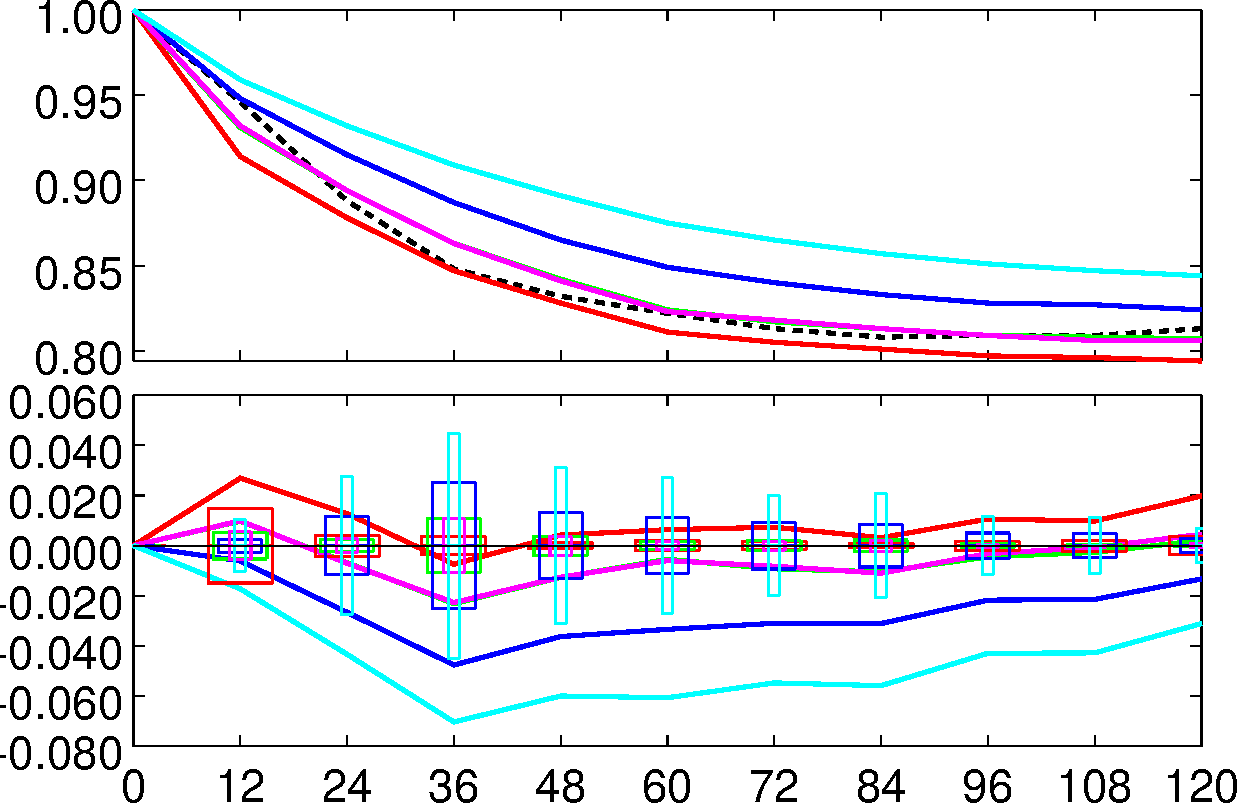
\includegraphics[width=0.3095\textwidth]{./figs/cap5/skill_prevs120h/0012z/ACOR_umes925_tropic-0012z-crop.pdf}
        }
        \subfigure[$q$ 925 hPa - 00 e 12Z, HS]{
            \label{fig:q925hs0012}
            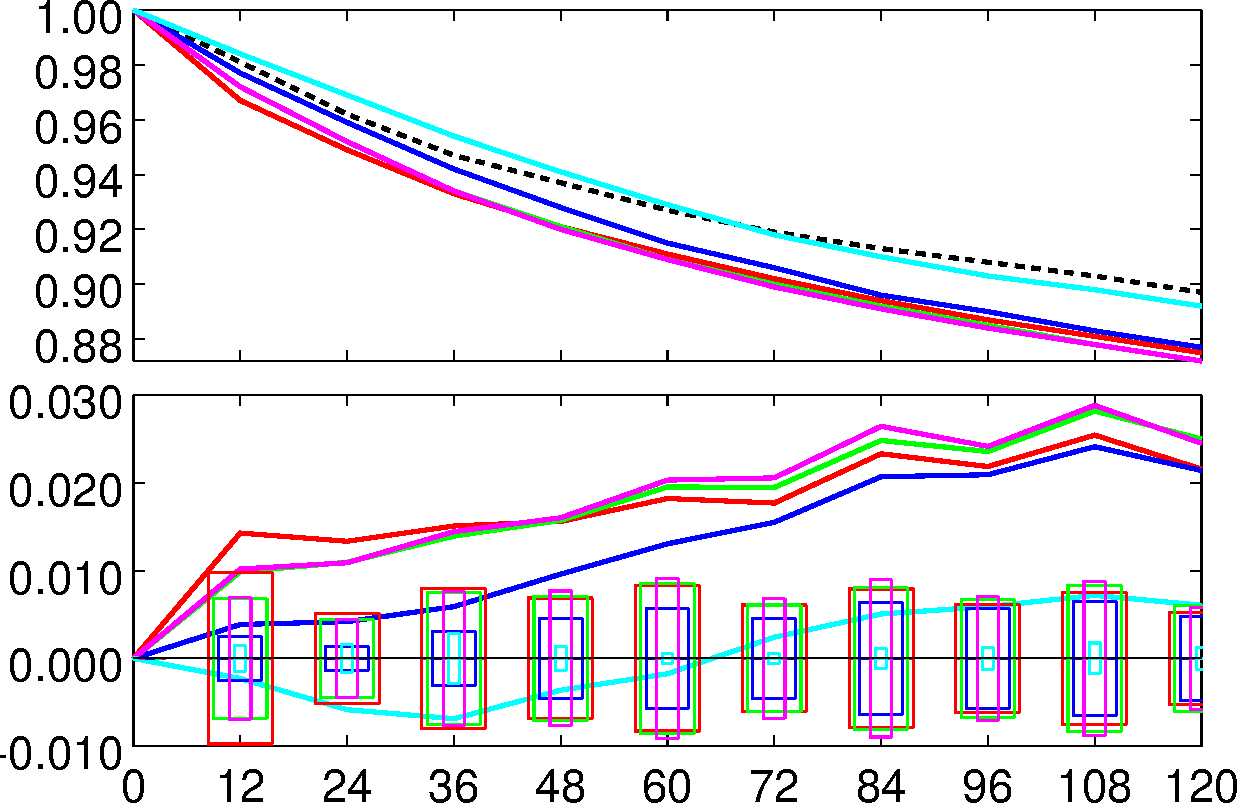
\includegraphics[width=0.3095\textwidth]{./figs/cap5/skill_prevs120h/0012z/ACOR_umes925_hemsul-0012z-crop.pdf}
        }\\
        \subfigure[$T$ 850 hPa - 00 e 12Z, HN]{
            \label{fig:T850hn0012}
            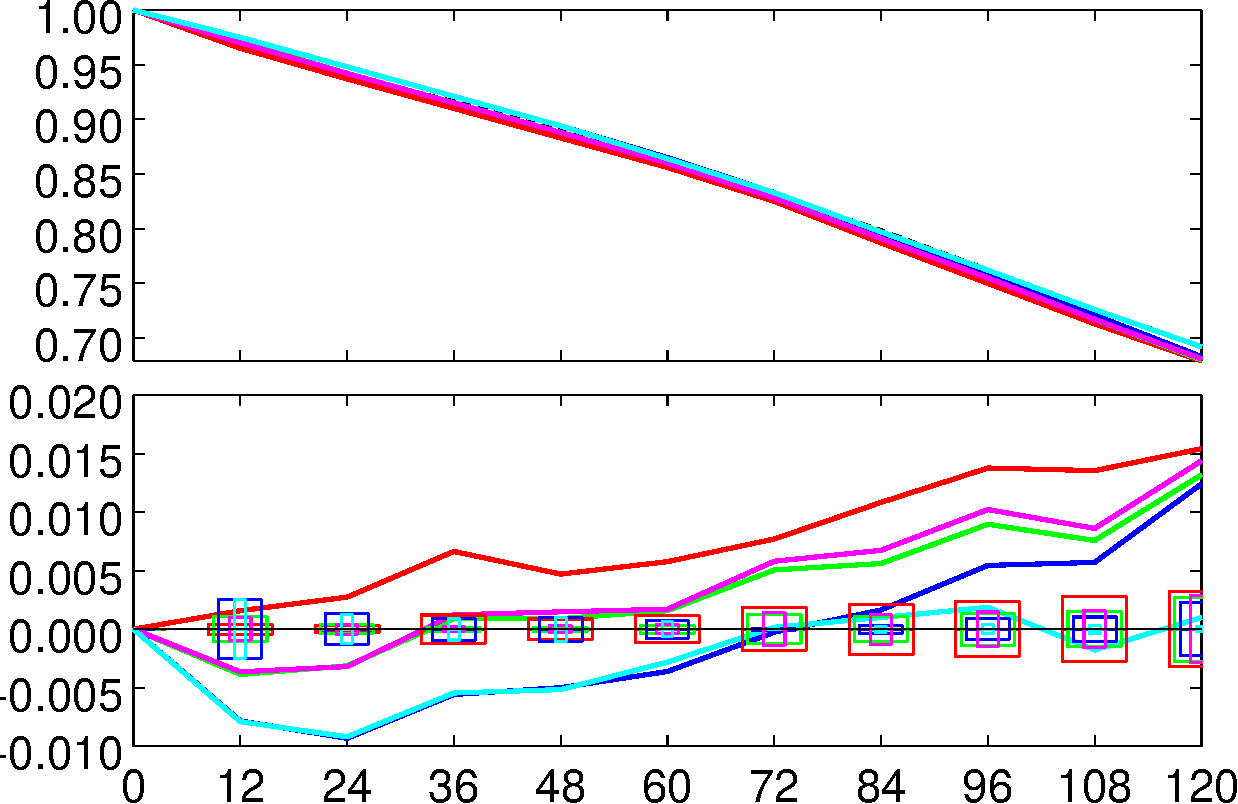
\includegraphics[width=0.3095\textwidth]{./figs/cap5/skill_prevs120h/0012z/ACOR_temp850_hnorte-0012z-crop.pdf}
        }
        \subfigure[$T$ 850 hPa - 00 e 12Z, TR]{
          \label{fig:T850tr0012}
          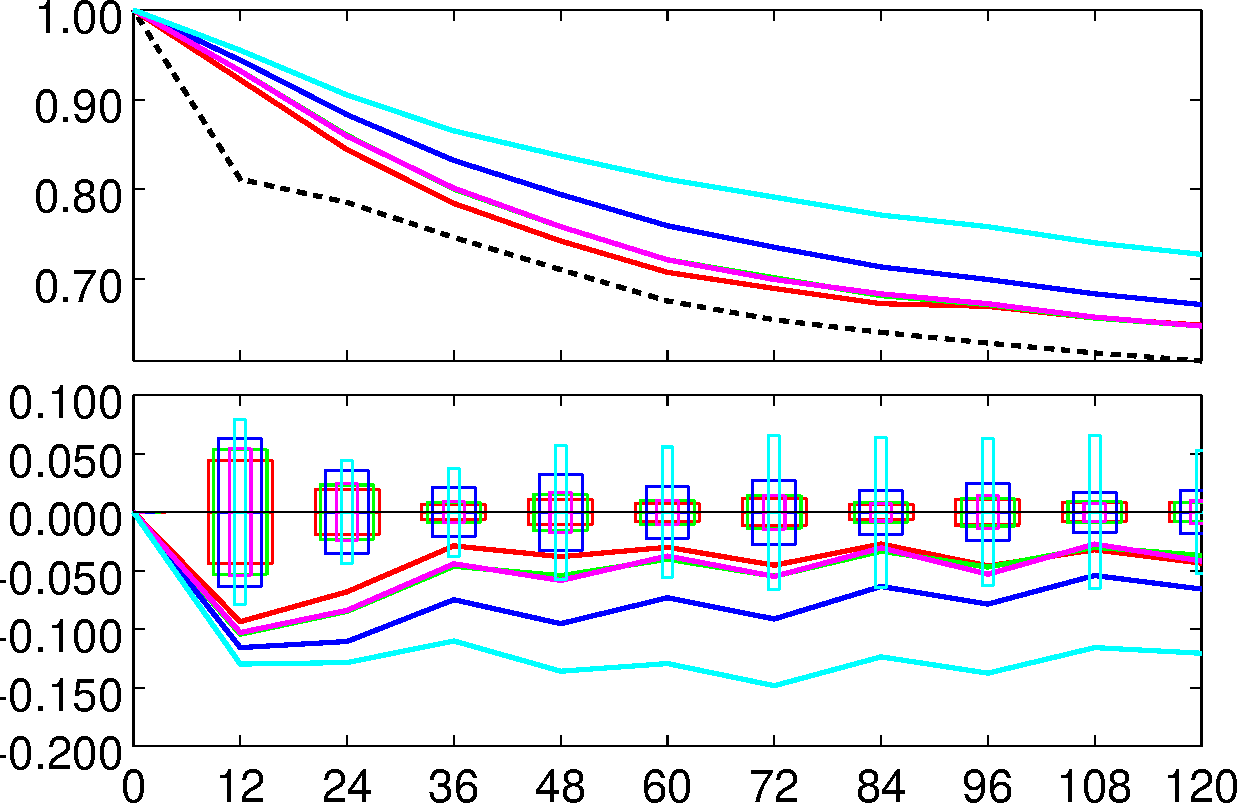
\includegraphics[width=0.3095\textwidth]{./figs/cap5/skill_prevs120h/0012z/ACOR_temp850_tropic-0012z-crop.pdf}
        }
        \subfigure[$T$ 850 hPa - 00 e 12Z, HS]{
            \label{fig:T850hs0012}
            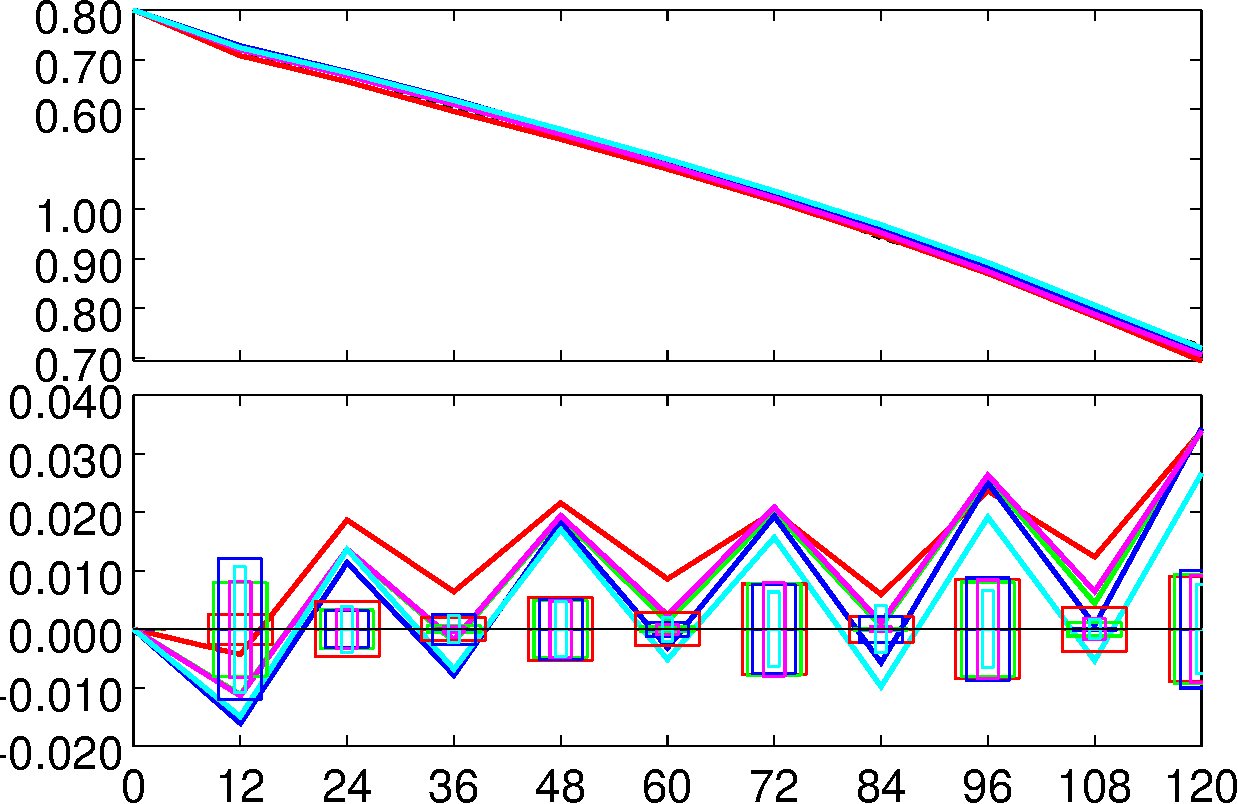
\includegraphics[width=0.3095\textwidth]{./figs/cap5/skill_prevs120h/0012z/ACOR_temp850_hemsul-0012z-crop.pdf}
        }\\
        \subfigure[$u$ 250 hPa - 00 e 12Z, HN]{
            \label{fig:u250hn0012}
            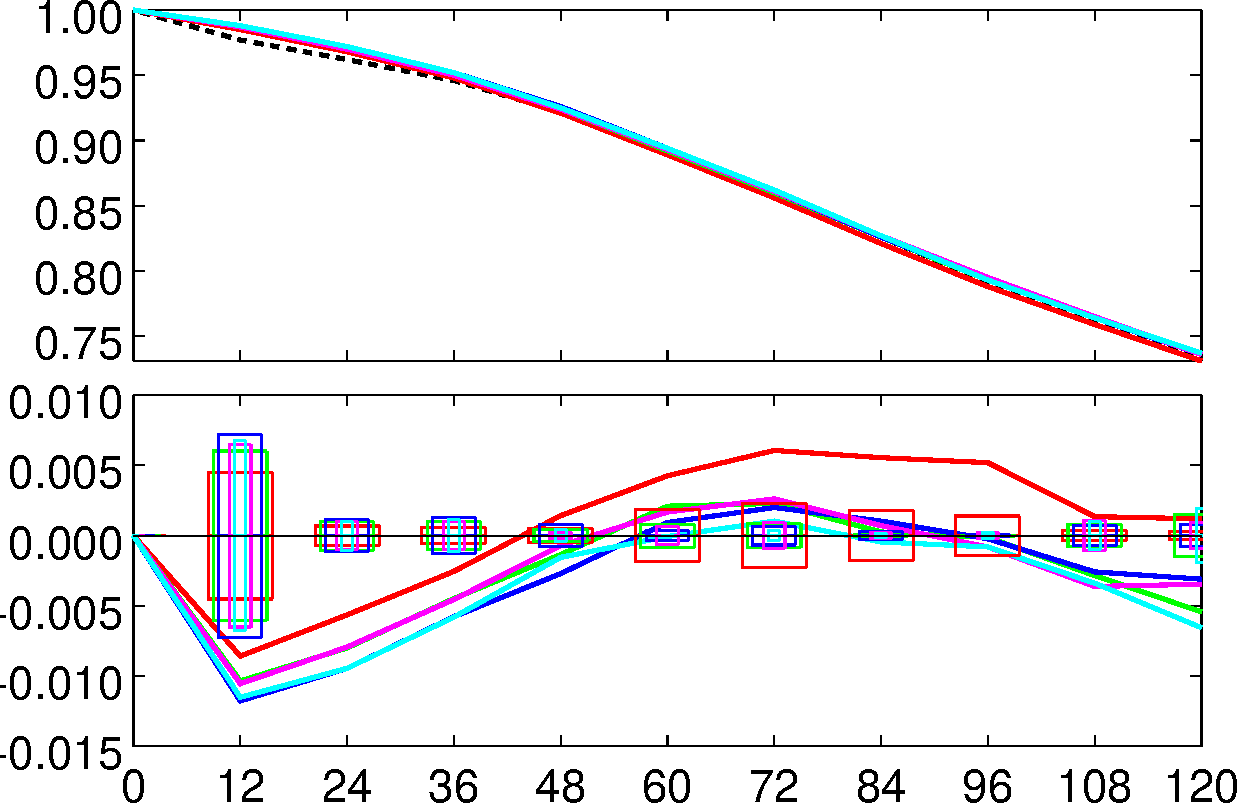
\includegraphics[width=0.3095\textwidth]{./figs/cap5/skill_prevs120h/0012z/ACOR_uvel250_hnorte-0012z-crop.pdf}
        }
        \subfigure[$u$ 250 hPa - 00 e 12Z, TR]{
          \label{fig:u250tr0012}
          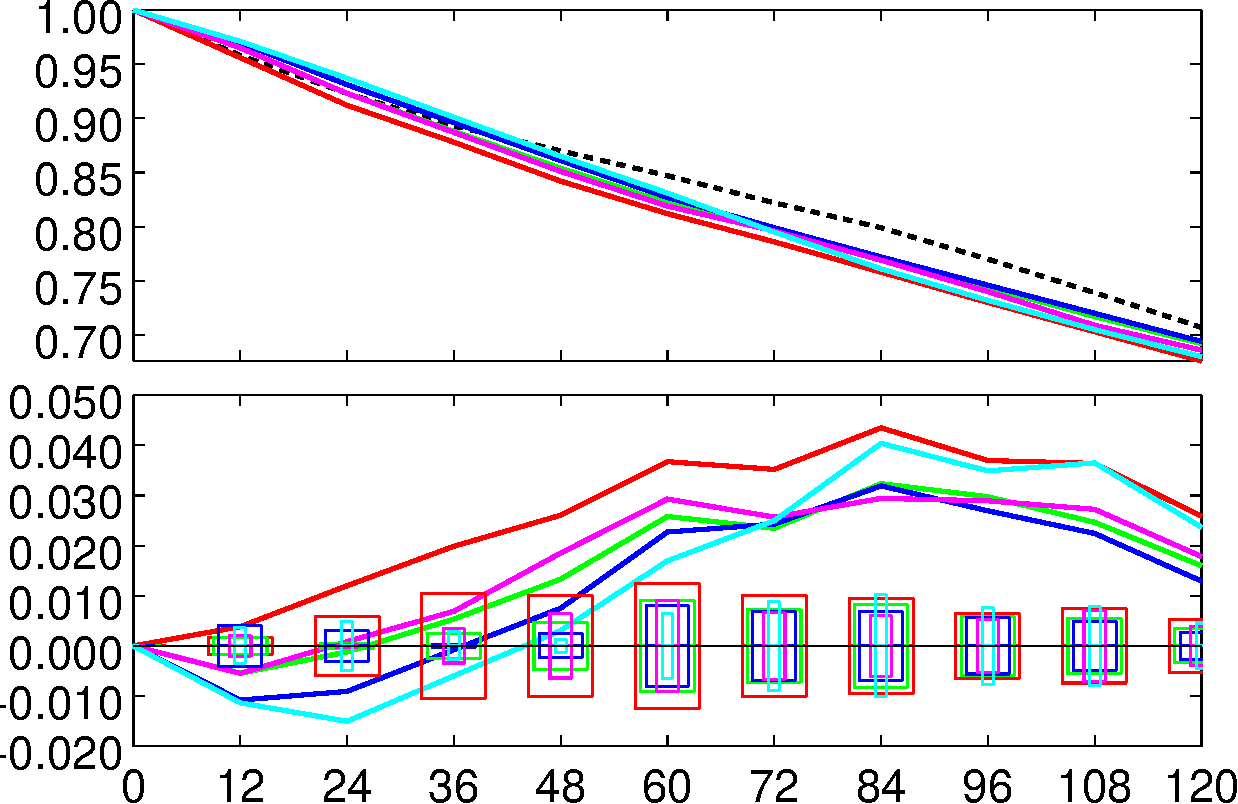
\includegraphics[width=0.3095\textwidth]{./figs/cap5/skill_prevs120h/0012z/ACOR_uvel250_tropic-0012z-crop.pdf}
        }
        \subfigure[$u$ 250 hPa - 00 e 12Z, HS]{
          \label{fig:u250hs0012}
          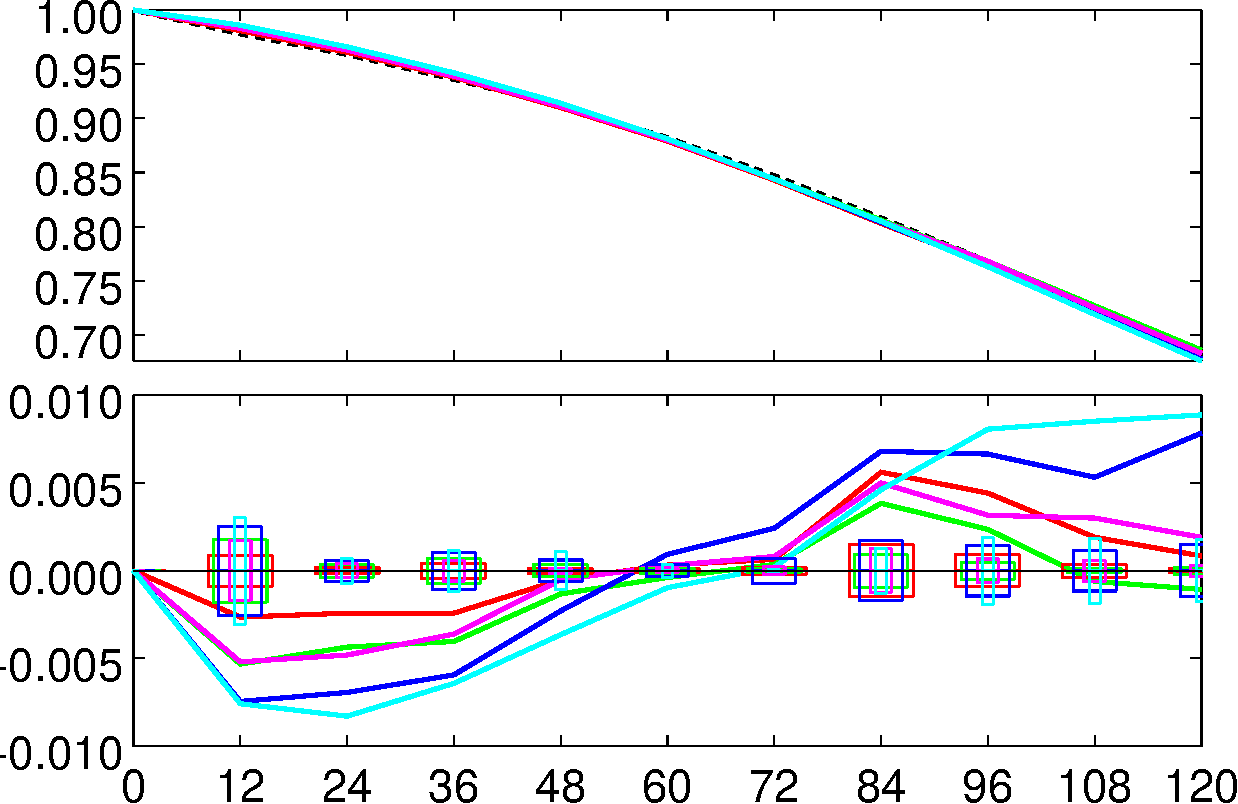
\includegraphics[width=0.3095\textwidth]{./figs/cap5/skill_prevs120h/0012z/ACOR_uvel250_hemsul-0012z-crop.pdf}
        }\\
        \subfigure[$z$ 500 hPa - 00 e 12Z, HN]{
            \label{fig:z500hn0012}
            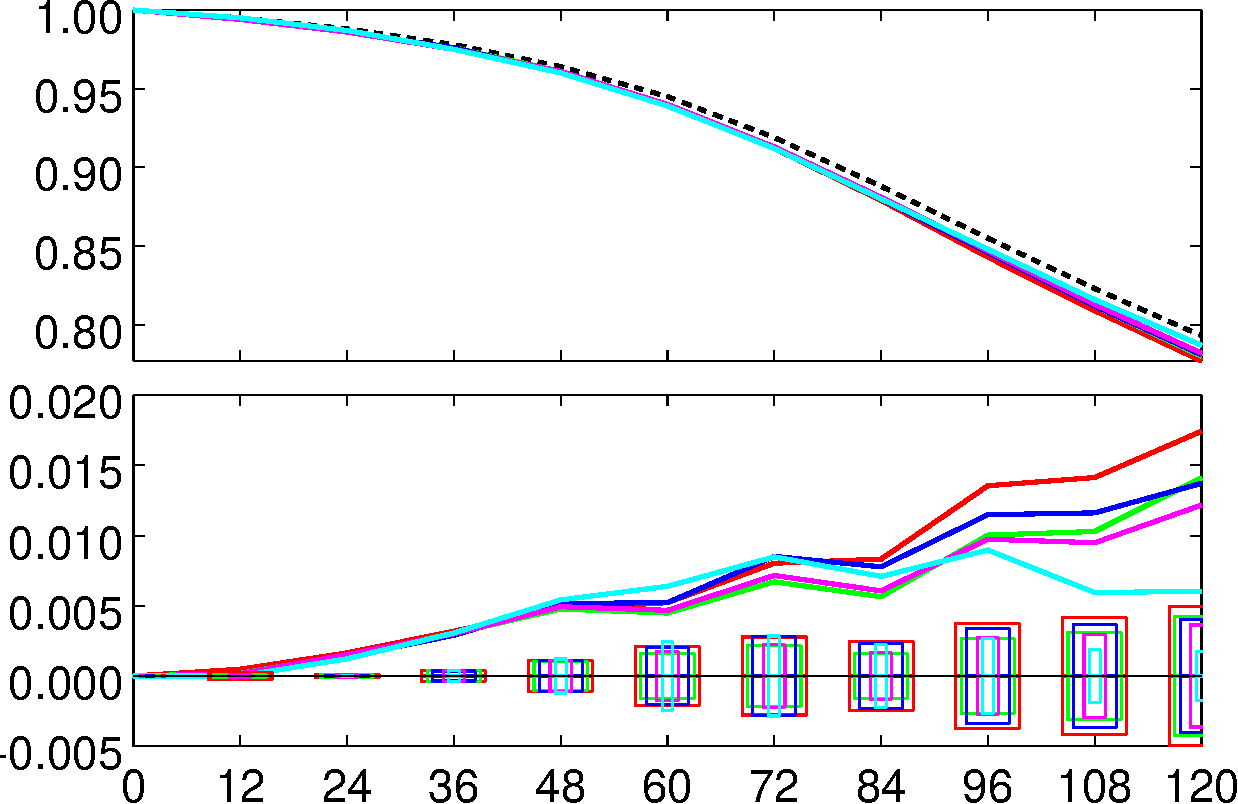
\includegraphics[width=0.3095\textwidth]{./figs/cap5/skill_prevs120h/0012z/ACOR_zgeo500_hnorte-0012z-crop.pdf}
        }
        \subfigure[$z$ 500 hPa - 00 e 12Z, TR]{
          \label{fig:z500tr0012}
          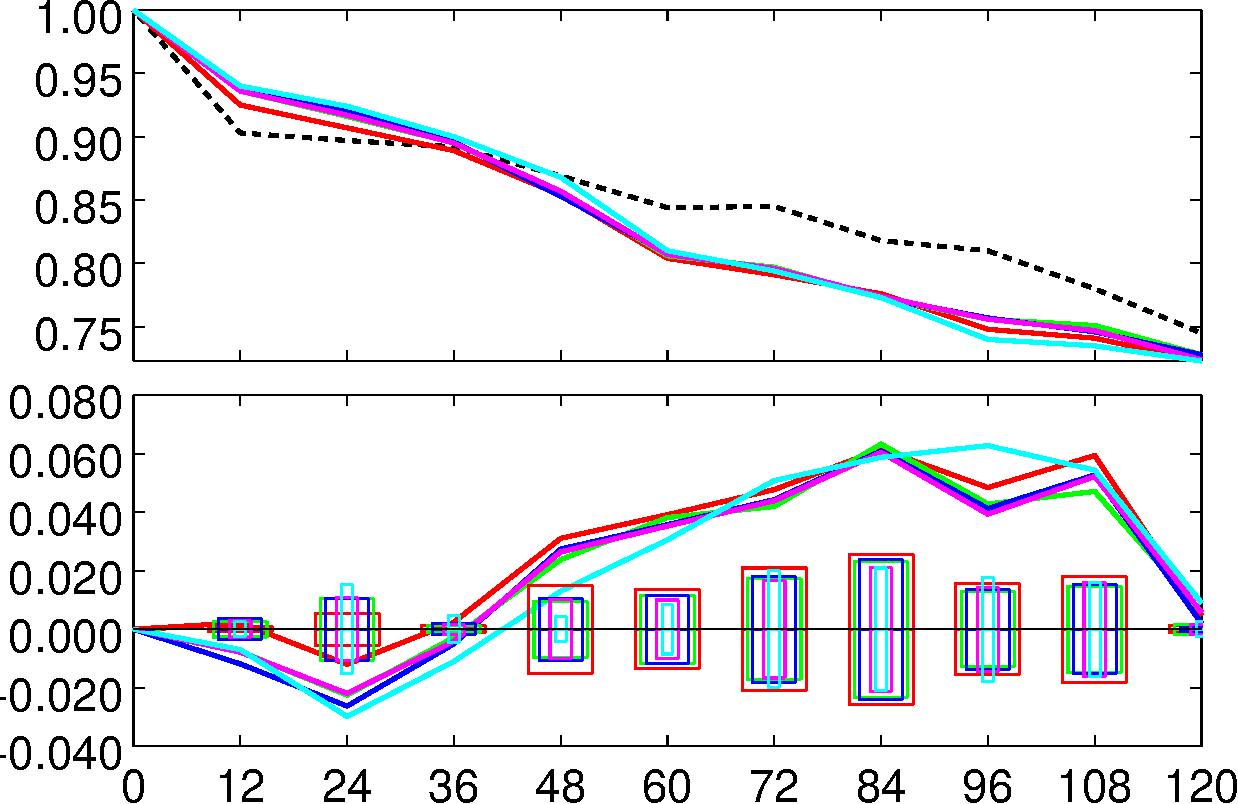
\includegraphics[width=0.3095\textwidth]{./figs/cap5/skill_prevs120h/0012z/ACOR_zgeo500_tropic-0012z-crop.pdf}
        }     
        \subfigure[$z$ 500 hPa - 00 e 12Z, HS]{
          \label{fig:z500hs0012}
          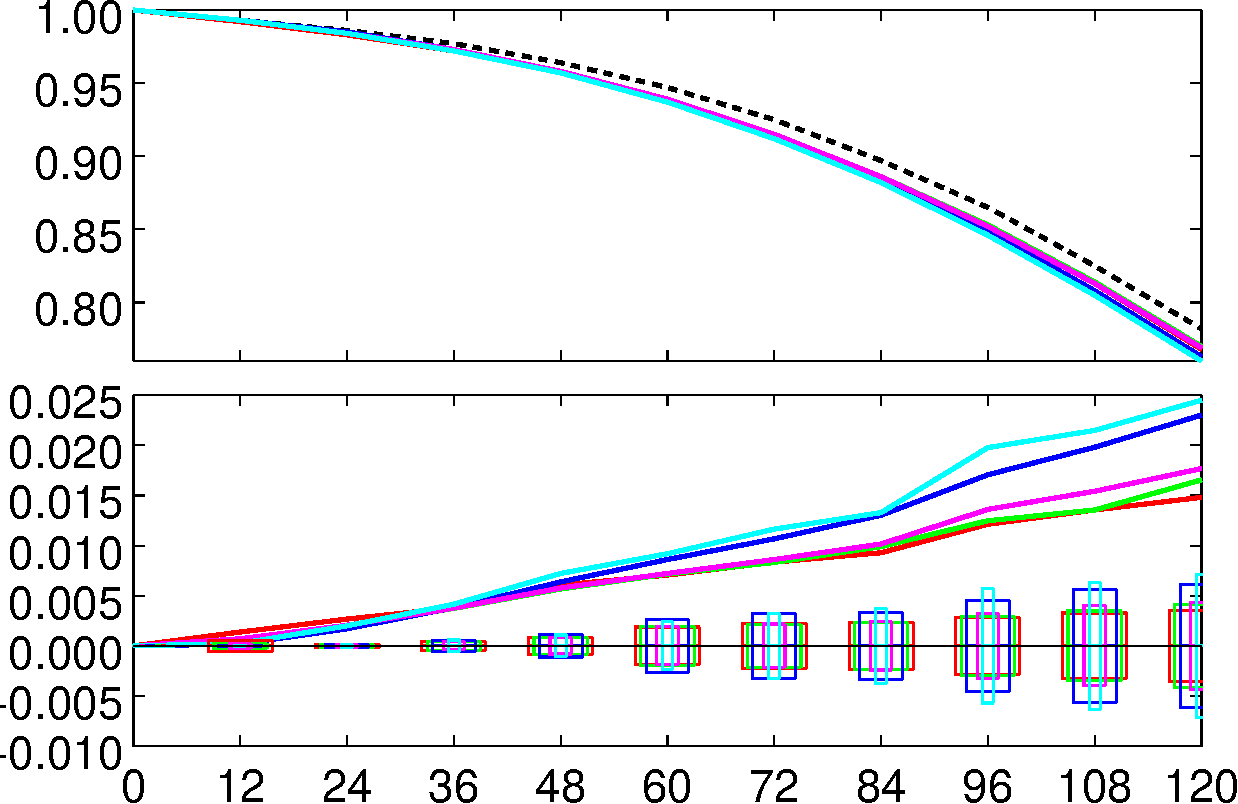
\includegraphics[width=0.3095\textwidth]{./figs/cap5/skill_prevs120h/0012z/ACOR_zgeo500_hemsul-0012z-crop.pdf}
        }        
    \end{center}
    \vspace{2mm}
    \legenda{As variáveis avaliadas são pressão em superfície ($psnm$), umidade em 925 hPa ($q925$), temperatura em 850 hPa ($T850$), vento zonal em 250hPa ($u250$) e altura geopotencial em 500 hPa ($z500$). As curvas pretas pontilhadas, indicam o experimento REF; em vermelho está representado o experimento 3DVar; em verde, o experimento EnKF50; em azul, EnKF75; em rosa, EnSRF50 e em verde água, EnSRF75.}
  \label{fig:skill_nh_tr_sh}
  \FONTE{Produção do autor.}
\end{figure}

A Figura \ref{fig:skill_gl_sa} apresenta a mesma avaliação da Figura \ref{fig:skill_nh_tr_sh}, mas para as regiões GL e AS. A região AS é de grande interesse para o CPTEC por ser a região alvo de previsões do Brasil. Nestas regiões, a mesma resposta dos experimentos EnKF75 e EnSRF50 foi encontrada, indicando que na região AS, as covariâncias do conjunto de previsões também tem um papel importante na determinação da habilidade de previsão do modelo BAMv0. Para a região GL, os índices de CA são semelhantes ao que foi encontrado para a região HN. Além disso, a CA para a variável $q925$ na região GL (Figura \ref{fig:q925gl0012}) mostra que as previsões obtidas com o experimento EnSRF75 (e também com o experimento EnKF75) foram boas para 120 horas, ficando próximo de 95\%. Neste caso, entretanto, o teste t-Student revelou que o experimento EnKF75 falha no teste da hipótese nula em 72 horas de previsão, quando a análise do experimento REF fez com que o modelo BAMv0 produzisse previsões com melhor correlação com a climatologia. As demais variáveis (i.e., $psnm$, $T850$, $u250$ e $z500$ (Figuras \ref{fig:psnmgl0012}, \ref{fig:T850gl0012}, \ref{fig:u250gl0012} e \ref{fig:z500gl0012} respectivamente) mostram índices de CA semelhantes em comparação com os resultados obtidos sobre a região HN. Para a região AS, bons resultados foram obtidos para $psnm$ (Figura \ref{fig:q925as0012}), para até 84 horas de previsão; $q925$ (Figura \ref{fig:psnmas0012}) com CA maior do que 85\% para 120 horas e $T850$ (Figura \ref{fig:T850as0012}) com CA de 80\% com os experimentos EnSRF75 até 72 horas de previsão e EnKF75 para até 60 horas de previsão. O vento zonal em 250 hPa ($u250$) e, especialmente, a altura geopotencial em $z500$ (Figuras \ref{fig:u250as0012} e \ref{fig:z500as0012}, respectivamente) não apresentaram bom desempenho. $z500$ nos experimentos EnKF75 e EnSRF75 não desempenharam como as demais variáveis. Para além de 84 horas de previsão, elas foram piores e os experimentos EnKF50, EnSRF50 e mesmo o experimento 3DVar, foram melhores.

Uma comparação entre os esquemas de análise utilizados nos experimentos, mostram que a análise da umidade dos experimentos EnKF75 e EnSRF50 apresentaram melhora em relação do experimento 3DVar. As Figuras \ref{fig:psnmhs0012}, \ref{fig:q925hs0012}, \ref{fig:T850hs0012}, \ref{fig:q925gl0012} e \ref{fig:T850as0012}, mostram que as previsões de umidade foram piores com os ciclos de assimilação de dados se comparados com o experimento REF. Para os experimentos com o sistema híbrido 3DVar, a matriz estática dos erro de previsão é a mesma utilizada também no experimento 3DVar. Isto pode ser um indicativo de que as covariâncias dos conjuntos de previsões tem um papel importante também na definição de como os incrementos de análise são aplicados durante a minimização da função custo variacional.

\begin{figure}[H]
    \vspace{2mm}
    \caption{Idem Figura \ref{fig:skill_nh_tr_sh}, mas para as regiões Global (GL) e América do Sul (AS).}
    \begin{center}
        \subfigure[$psnm$ - 00 e 12Z, GL]{
            \label{fig:psnmgl0012}
            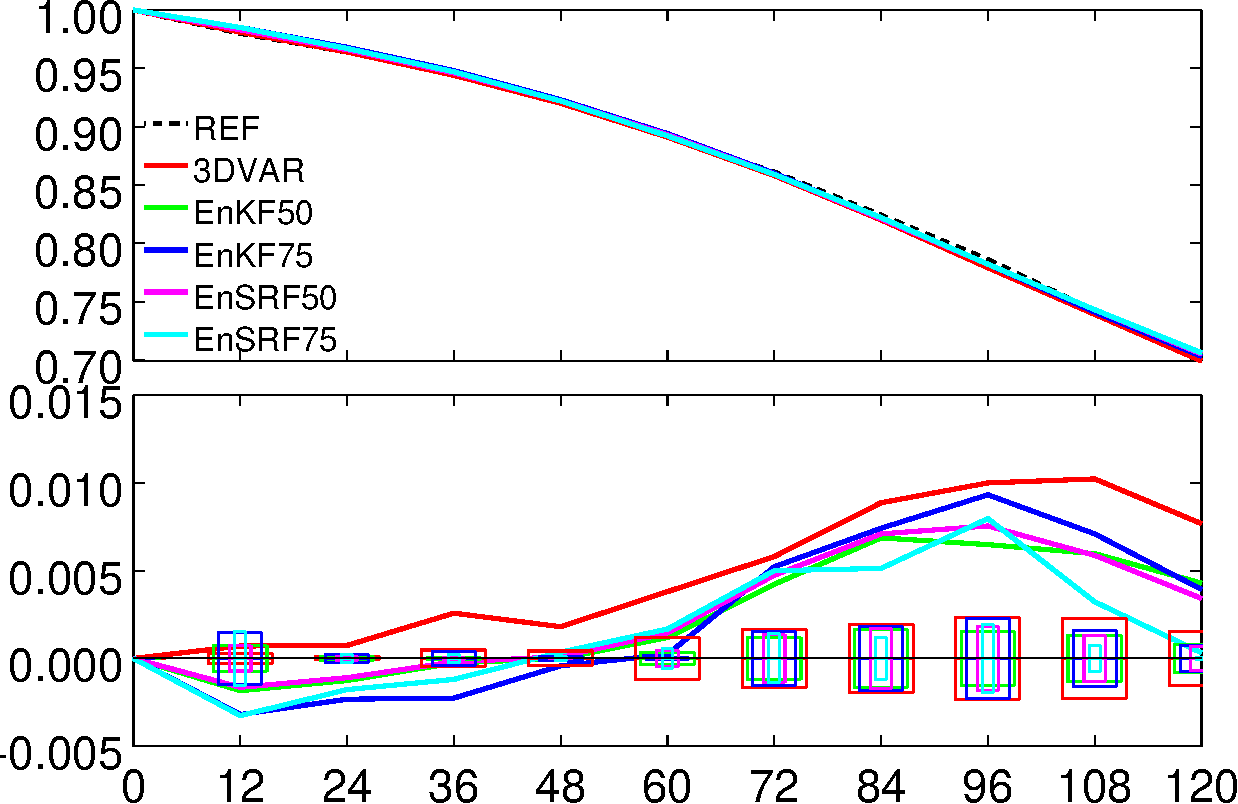
\includegraphics[width=0.3095\textwidth]{./figs/cap5/skill_prevs120h/0012z/ACOR_psnm000_global-0012z-legenda-crop.pdf}
        }
        \subfigure[$psnm$ - 00 e 12Z, AS]{
          \label{fig:psnmas0012}
          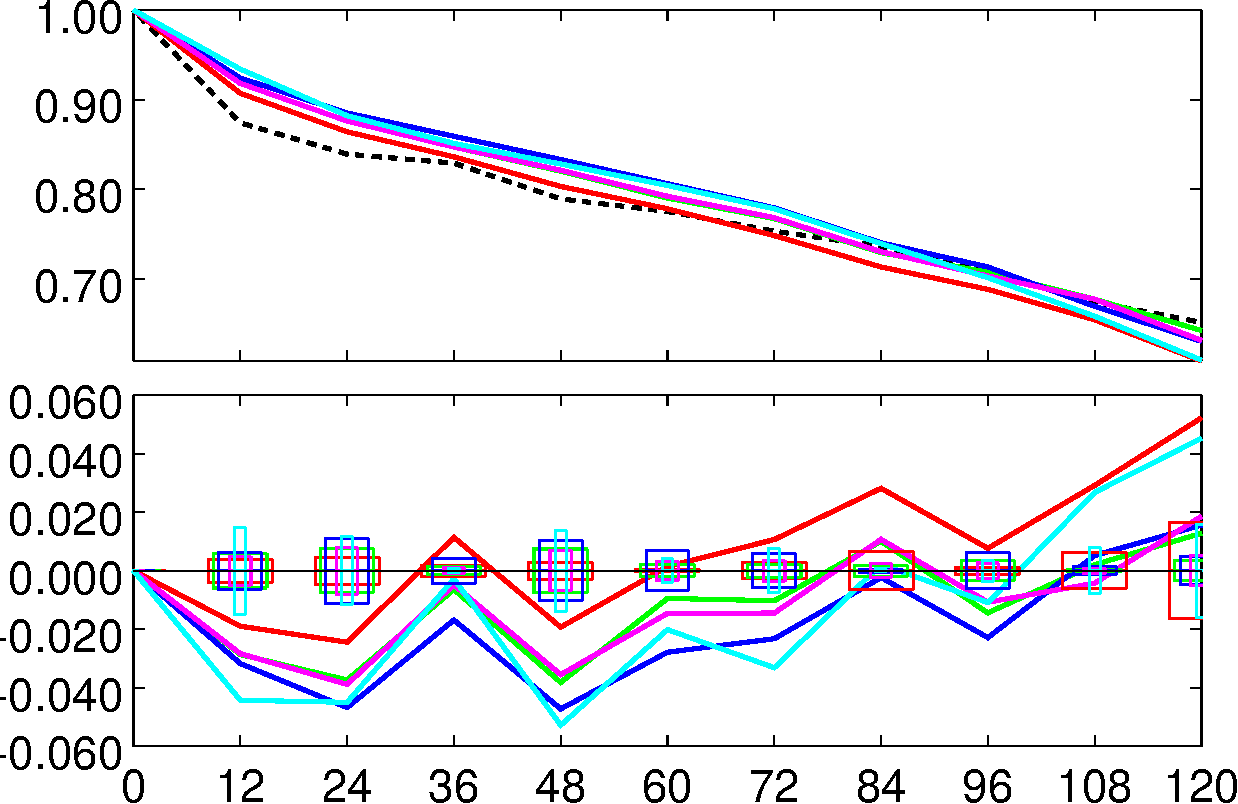
\includegraphics[width=0.3095\textwidth]{./figs/cap5/skill_prevs120h/0012z/ACOR_psnm000_amesul-0012z-crop.pdf}
        }\\     
        \subfigure[$q$ 925 hPa - 00 e 12Z, GL]{
            \label{fig:q925gl0012}
            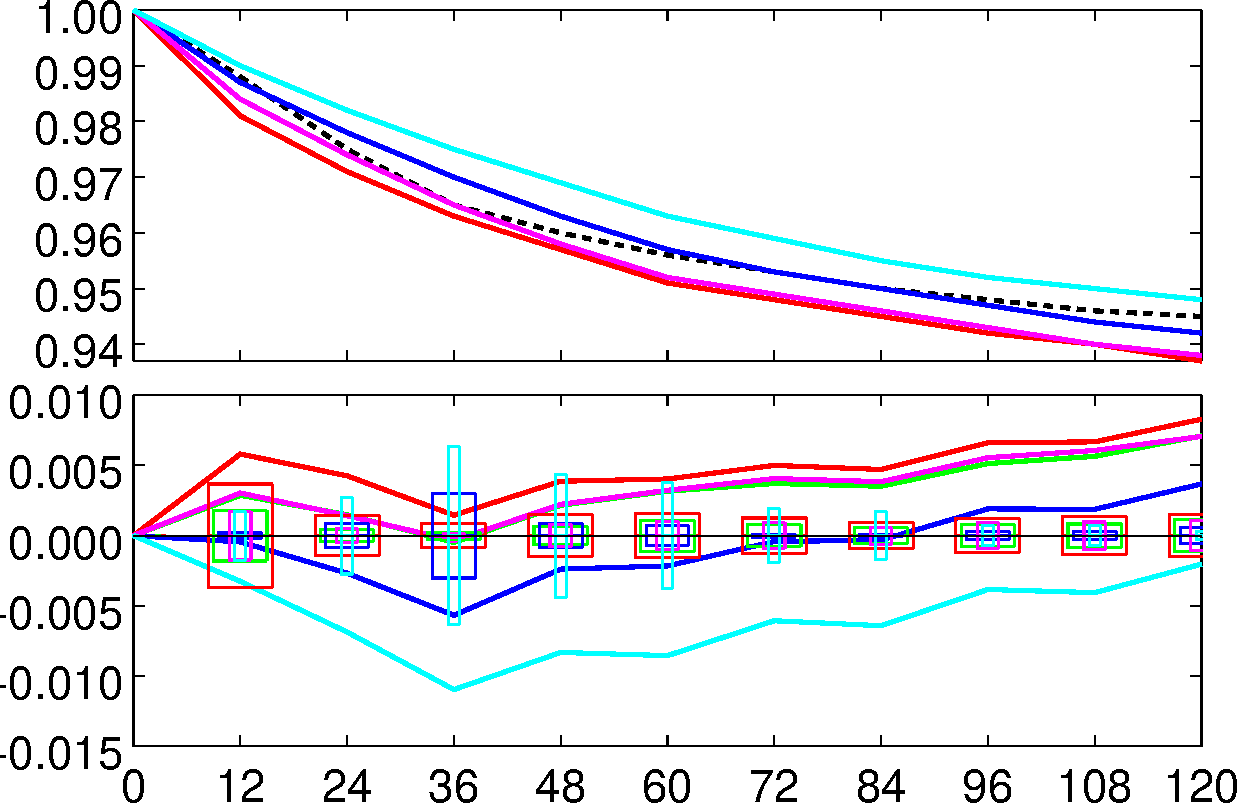
\includegraphics[width=0.3095\textwidth]{./figs/cap5/skill_prevs120h/0012z/ACOR_umes925_global-0012z-crop.pdf}
        }
        \subfigure[$q$ 925 hPa - 00 e 12Z, AS]{
          \label{fig:q925as0012}
          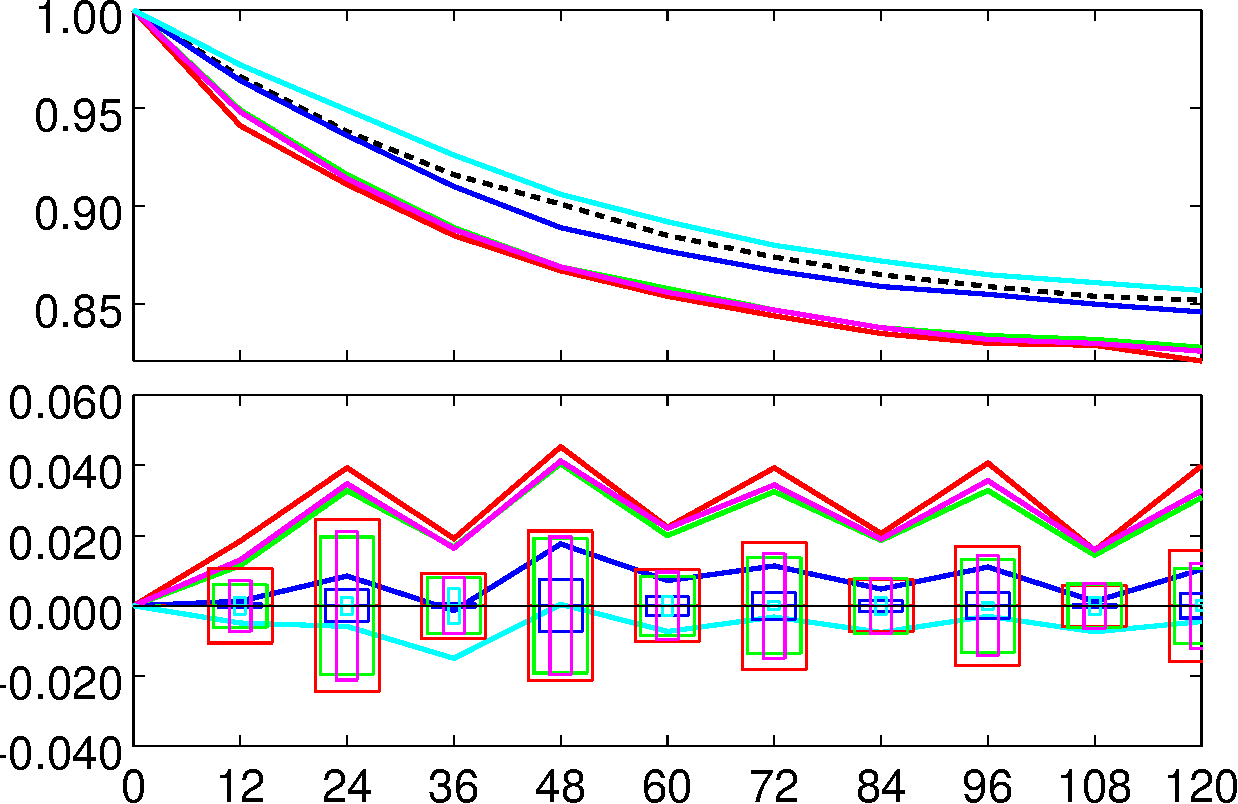
\includegraphics[width=0.3095\textwidth]{./figs/cap5/skill_prevs120h/0012z/ACOR_umes925_amesul-0012z-crop.pdf}
        }\\
        \subfigure[$T$ 850 hPa - 00 e 12Z, GL]{
            \label{fig:T850gl0012}
            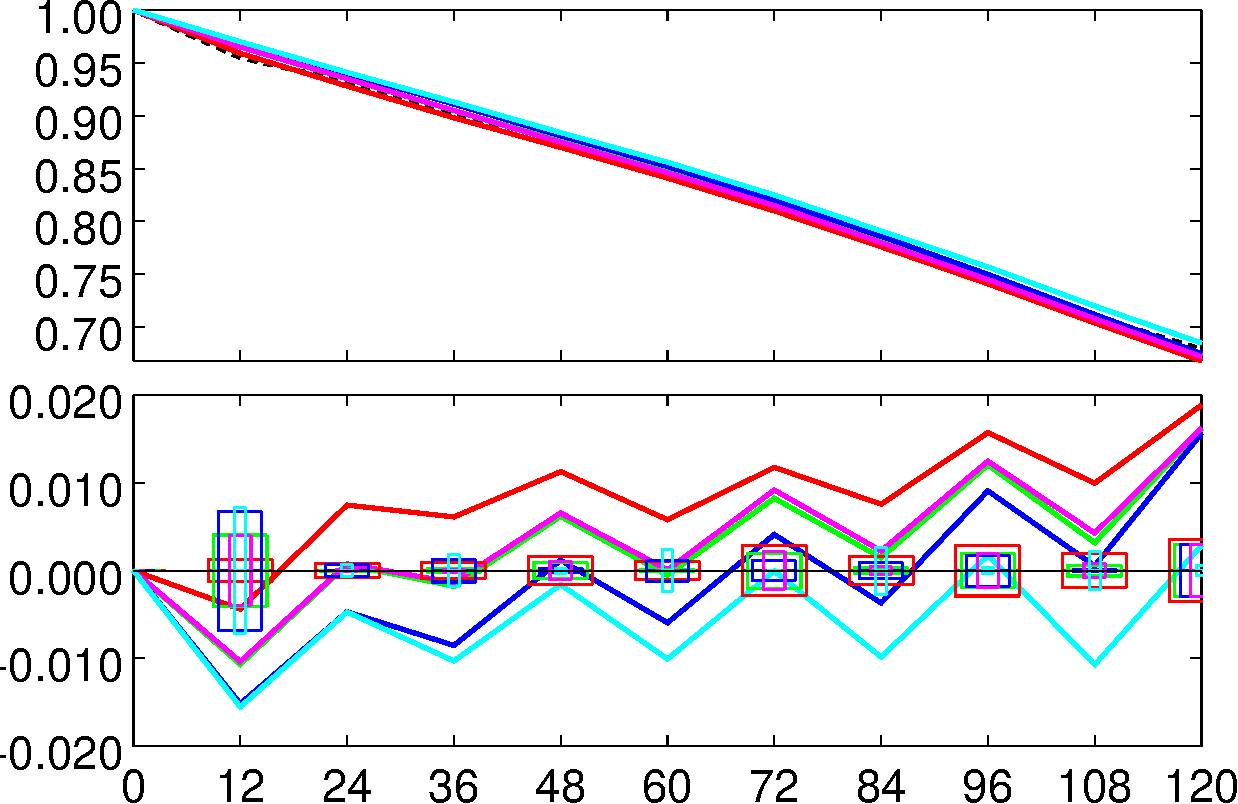
\includegraphics[width=0.3095\textwidth]{./figs/cap5/skill_prevs120h/0012z/ACOR_temp850_global-0012z-crop.pdf}
        }
        \subfigure[$T$ 850 hPa - 00 e 12Z, AS]{
          \label{fig:T850as0012}
          \includegraphics[width=0.3095\textwidth]{./figs/cap5/skill_prevs120h/0012z/ACOR_temp850_amesul-0012z-crop.pdf}
        }\\
        \subfigure[$u$ 250 hPa - 00 e 12Z, GL]{
            \label{fig:u250gl0012}
            \includegraphics[width=0.3095\textwidth]{./figs/cap5/skill_prevs120h/0012z/ACOR_uvel250_global-0012z-crop.pdf}
        }
        \subfigure[$u$ 250 hPa - 00 e 12Z, AS]{
          \label{fig:u250as0012}
          \includegraphics[width=0.3095\textwidth]{./figs/cap5/skill_prevs120h/0012z/ACOR_uvel250_amesul-0012z-crop.pdf}
        }\\
        \subfigure[$z$ 500 hPa - 00 e 12Z, GL]{
            \label{fig:z500gl0012}
            \includegraphics[width=0.3095\textwidth]{./figs/cap5/skill_prevs120h/0012z/ACOR_zgeo500_global-0012z-crop.pdf}
        }
        \subfigure[$z$ 500 hPa - 00 e 12Z, AS]{
          \label{fig:z500as0012}
          \includegraphics[width=0.3095\textwidth]{./figs/cap5/skill_prevs120h/0012z/ACOR_zgeo500_amesul-0012z-crop.pdf}
        }       
    \end{center}
    \vspace{2mm}
    \legenda{}
  \label{fig:skill_gl_sa}
  \FONTE{Produção do autor.}
\end{figure}

\subsection{Avaliação das Previsões de 24 horas de Precipitação}
\label{sec:aval_prec}

As previsões de precipitação de 24 horas produzidas a partir das análises dos experimentos REF, 3DVar puro e híbridos 3DVar foram avaliadas. A Figura \ref{fig:gpcpprec24h12z} mostra a média mensal para Janeiro de 2013 da precipitação observada do \textit{Global Precipitation Climatology Project v2.2} (GPCPv2.2) com resolução espacial de 2,5$^{\circ}$ \cite{adleretal/2003} e as Figuras \ref{fig:refprec24h12z}, \ref{fig:3dvarprec24h12z}, \ref{fig:enkf50prec24h12z}, \ref{fig:enkf75prec24h12z}, \ref{fig:ensrf50prec24h12z} e \ref{fig:ensrf75prec24h12z} mostram a precipitação de 24 horas prevista - representada como média mensal, dos experimentos realizados REF, 3DVar puro e híbridos 3DVar. A comparação entre as médias mensais das precipitações de 24 horas e o GPCPv2.2 é válida no horário das 12Z e os dados em ponto de grade dos modelos foram interpolados para 2,5$^{\circ}$ para coincidir com a resolução dos dados observados do GPCPv2.2. O campo da média mensal de precipitação do GPCPv2.2 mostra as principais características da precipitação tropical e subtropical, com a maior parte da precipitação distribuída sobre a região tropical (entre 30S e 30N).

Na Figura \ref{fig:medprecobs_exps}, com excessão do experimento REF, todos os experimentos foram realizados com ciclos de assimilação de dados, utilizando todos os dados observados da Tabela \ref{tab:mobs}, a mesma resolução e com as mesmas configurações do modelo de circulação geral (tal como definido na Tabela \ref{tab:model}). Todos os experimentos mostram as características da precipitação convectiva e de larga escala e a Figura \ref{fig:gpcpprec24h12z} é usada como referência para uma avaliação da intensidade e distribuição das médias espacial e temporal. A Tabela \ref{tab:prec_aave_exps} apresenta os valores das médias espaciais das médias do período, para o GPCPvv2.2 e os experimentos realizados.

\begin{figure}[H]
    \vspace{-4mm}
    \caption{Médias espaciais das previsões de precipitação de 24 horas (em mm/dia) válido para Janeiro de 2013 às 12Z.}
    \begin{center}
        \subfigure[GPCP $prec$ 24 h - 12Z]{
            \label{fig:gpcpprec24h12z}
            \includegraphics[width=0.477\textwidth]{./figs/cap5/aval_prec24h/medias_espaciais/precip_gpcp_3dvar_3densvar-new_prec_medias-artigo-gpcp2-crop.pdf} 
        }\\ 
        \subfigure[REF $prec$ 24 h - 12Z]{
          \label{fig:refprec24h12z}
          \includegraphics[width=0.477\textwidth]{./figs/cap5/aval_prec24h/medias_espaciais/precip_gpcp_3dvar_3densvar-new_prec_medias-artigo-ref2-crop.pdf}
        }
        \subfigure[3DVar $prec$ 24 h - 12Z]{
          \label{fig:3dvarprec24h12z}
          \includegraphics[width=0.477\textwidth]{./figs/cap5/aval_prec24h/medias_espaciais/precip_gpcp_3dvar_3densvar-new_prec_medias-artigo-3dvar2-crop.pdf}
        }\\       
        \subfigure[EnKF50 $prec$ 24 h - 12Z]{
          \label{fig:enkf50prec24h12z}
          \includegraphics[width=0.477\textwidth]{./figs/cap5/aval_prec24h/medias_espaciais/precip_gpcp_3dvar_3densvar-new_prec_medias-artigo-enkf502-crop.pdf}
        }
        \subfigure[EnKF75 $prec$ 24 h - 12Z]{
          \label{fig:enkf75prec24h12z}
          \includegraphics[width=0.477\textwidth]{./figs/cap5/aval_prec24h/medias_espaciais/precip_gpcp_3dvar_3densvar-new_prec_medias-artigo-enkf752-crop.pdf}
        }\\  
        \subfigure[EnSRF50 $prec$ 24 h - 12Z]{
          \label{fig:ensrf50prec24h12z}
          \includegraphics[width=0.477\textwidth]{./figs/cap5/aval_prec24h/medias_espaciais/precip_gpcp_3dvar_3densvar-new_prec_medias-artigo-ensrf502-crop.pdf}
        }
        \subfigure[EnSRF75 $prec$ 24 h - 12Z]{
          \label{fig:ensrf75prec24h12z}
          \includegraphics[width=0.477\textwidth]{./figs/cap5/aval_prec24h/medias_espaciais/precip_gpcp_3dvar_3densvar-new_prec_medias-artigo-ensrf752-crop.pdf}
        }\\            
        \includegraphics[width=0.04\textwidth,angle=-90]{./figs/cap5/aval_prec24h/medias_espaciais/cbar_prec_exps-crop.pdf}
    \end{center}
    \vspace{2mm}
    \legenda{Em \subref{fig:gpcpprec24h12z} precipitação do GPCPv2.2; \subref{fig:refprec24h12z} experimento REF; \subref{fig:3dvarprec24h12z} 3DVar; \subref{fig:enkf50prec24h12z} EnKF50; \subref{fig:enkf75prec24h12z} EnKF75; \subref{fig:ensrf50prec24h12z} EnSRF50; \subref{fig:ensrf75prec24h12z} EnSRF75.}
    \label{fig:medprecobs_exps}
    \FONTE{Produção do autor.}
\end{figure}

As previsões de precipitação dos experimentos, apresentam distribuição espacial coerente em comparação com a média mensal do GPCPv2.2 (Figura \ref{fig:gpcpprec24h12z}). Ressalta-se que a configuração do modelo para a condensação de larga escala, convecção \textit{Cumulus} e difusões horizontal e vertical foram mantidas iguais, portanto, as diferenças observadas são devidas apenas as análises utilizadas. As principais diferenças entre as previsões de precipitação dos experimentos estão mais relacionadas a intensidade da precipitação. A Figura \ref{fig:gpcpprec24h12z}, mostra a média mensal da precipitação de 24 horas resultante do modelo BAMv0 inicializado com a análise do NCEP (experimento REF). Em comparação com os demais experimentos (incluindo a precipitação de referência do GPCPv2.2), o modelo BAMv0 apresentou tendência a produzir mais precipitação convectiva sobre a região tropical. A média espacial da média temporal resulta em 2,9718 mm/mês, contabilizando a maior quantidade de precipitação entre os experimentos realizados, sendo maior até do que a precipitação de referência do GPCPv2.2 (2,7197 mm/mês). Por outro lado, todos os experimentos com assimilação de dados, produziram precipitação com distribuição menos concentrada e médias espaciais mais razoáveis. A média espacial do experimento EnSRF50 (Figura \ref{fig:enkf50prec24h12z}) é a que mais se aproxima com o valor apresentado pelo GPCPv2.2, embora os demais experimentos com assimilação de dados tenham distribuído a precipitação convectiva de forma mais coerente (em relação ao GPCPv2.2).

\begin{table}[H]
\caption{Médias espaciais sobre a região Global (GL) para a referência (GPCPv2.2) e os experimentos realizados das previsões de 24 horas da precipitação total às 12Z (em mm/mês). Em azul, estão indicados os experimentos cujas médias são mais próximas a média de precipitação da referência.}
\begin{center}
\begin{adjustbox}{max width=\textwidth}
%\renewcommand{\arraystretch}{1.5}
\begin{tabular}{rc}
\toprule
\toprule
 & $\mu$ \\
\midrule
\textbf{GPCPv2.2}    & 2,7197 \\
\textbf{REF}     & 2,9718 \\
\textbf{3DVar}   & 2,6098 \\
\textbf{EnKF50}  & \color{blue}{2,7034} \\
\textbf{EnKF75}  & 2,6730 \\
\textbf{EnSRF50} & \color{blue}{2,7045} \\
\textbf{EnSRF75} & 2,5618 \\ 
\bottomrule                                         
\end{tabular}
\end{adjustbox}
\end{center}
\label{tab:prec_aave_exps}
\end{table}

A quantidade exagerada de precipitação produzida pelo experimento REF (Figura \ref{fig:refprec24h12z}) pode ser devida ao fato de que este experimento foi feito simplesmente integrando-se o modelo BAMv0 com as análises do NCEP, embora a suavização da topografia e inicialização com modos normais para cada análise no período de avaliação tenham sido feitas neste experimento em específico. Os experimentos com ciclos de assimilação de dados, com excessão do experimento EnSRF75 (Figura \ref{fig:ensrf75prec24h12z}) - o qual resultou na menor média mensal, mostrou-se estar bem condicionado as opções escolhidas para as previsões.

Para se tentar entender e identificar as regiões onde os experimentos acumularam mais ou menos a precipitação, as Figuras \ref{fig:medprecobs_gl} e \ref{fig:medprecobs_hntrhsas} apresentam as séries temporais das médias espaciais para cada experimento, incluindo o GPCP sobre as regiões GL, HN, TR, HS e AS. Nestas figuras, o GPCPv1.2 1DD (1 Degree Daily - \citeonline{huffmanetal/2001}) foi utilizado como dado observado e este foi interpolado para a grade das análises dos experimentos (com 1,875$^{\circ}$. Em adição as Figuras \ref{fig:medprecobs_gl} e \ref{fig:medprecobs_hntrhsas}, a Tabela \ref{tab:prec_aave_regs_sh_tr_sh} mostra as médias espaciais ($\mu$) e os desvios-padrão ($\sigma$) para cada experimento (incluindo o dado interpolado do GPCPv1.2) nas regiões avaliadas indicadas.

\begin{figure}[H]
    \vspace{2mm}
    \caption{Médias espaciais das previsões de precipitação de 24 horas (em mm/dia) válido para Janeiro de 2013 às 12Z, para a região GL (Global).}
    \begin{center}
      \includegraphics[width=1\textwidth]{./figs/cap5/aval_prec24h/series_temporais/precip_gpcp_3dvar_3densvar-new_prec_media-artigo-gl-crop.pdf}
      \includegraphics[width=0.75\textwidth]{./figs/cap5/aval_prec24h/series_temporais/precip_gpcp_3dvar_3densvar-new_prec_media-artigo-cbar-crop.pdf}
    \end{center}
    \vspace{2mm}
    \legenda{A precipitação dos experimentos é comparada com a precipitação observada do GPCPv1.2.}
    \label{fig:medprecobs_gl}
    \FONTE{Produção do autor.}
\end{figure}

\begin{figure}[H]
    \vspace{2mm}
    \caption{Idem Figura \ref{fig:medprecobs_gl}, para as regiões \subref{fig:sprec12hn} precipitação para todo o Hemisfério Norte (HN); \subref{fig:sprec12tr} Trópicos (TR); \subref{fig:sprec12hs} Hemisfério Sul (HS); \subref{fig:sprec12as} América do Sul (AS).}
    \begin{center}
        \subfigure[$prec$ 24 h - 12Z, HN]{
          \label{fig:sprec12hn}
          \includegraphics[width=1\textwidth]{./figs/cap5/aval_prec24h/series_temporais/precip_gpcp_3dvar_3densvar-new_prec_media-artigo-hn-crop.pdf}
        }\\     
        \subfigure[$prec$ 24 h - 12Z, TR]{
          \label{fig:sprec12tr}
          \includegraphics[width=1\textwidth]{./figs/cap5/aval_prec24h/series_temporais/precip_gpcp_3dvar_3densvar-new_prec_media-artigo-tr-crop.pdf}
        }\\       
        \subfigure[$prec$ 24 h - 12Z, HS]{
          \label{fig:sprec12hs}
          \includegraphics[width=1\textwidth]{./figs/cap5/aval_prec24h/series_temporais/precip_gpcp_3dvar_3densvar-new_prec_media-artigo-hs-crop.pdf}
        }\\
        \subfigure[$prec$ 24 h - 12Z, AS]{
          \label{fig:sprec12as}
          \includegraphics[width=1\textwidth]{./figs/cap5/aval_prec24h/series_temporais/precip_gpcp_3dvar_3densvar-new_prec_media-artigo-as-crop.pdf}
        }\\
        \includegraphics[width=0.75\textwidth]{./figs/cap5/aval_prec24h/series_temporais/precip_gpcp_3dvar_3densvar-new_prec_media-artigo-cbar-crop.pdf}
    \end{center}
    \vspace{2mm}
    \legenda{A precipitação dos experimentos é comparada com a precipitação observada do GPCPv1.2.}
    \label{fig:medprecobs_hntrhsas}
    \FONTE{Produção do autor.}
\end{figure}

Em contraste com o que foi encontrado com a análise da distribuição espacial dos campos de precipitação dos experimentos na Figura \ref{fig:medprecobs_exps}, a série temporal com as médias espaciais mostradas nas Figuras \ref{fig:medprecobs_gl} e \ref{fig:medprecobs_hntrhsas}, indicam que - com excessão da região HN (Figura \ref{fig:sprec12hn}), todos os experimentos apresentaram dificuldades em reproduzir a precipitação observada do GPCPv1.2 em previsões de 24 horas. Deficiências podem ser notadas em relação a amplitude (máximos e mínimos) e em relação a média. Em alguns casos específicos, a precipitação prevista foi praticamente igual aos valores médios observados - e.g., o experimento EnSRF75 na região TR (Figura \ref{fig:sprec12tr}) se igualou ao GPCPv1.2 durante alguns períodos do mês. Este resultado está de acordo com o que foi encontrado na análise da habilidade do modelo na previsão de até 120 horas (Figuras \ref{fig:skill_nh_tr_sh} e \ref{fig:skill_gl_sa}), mostrando que entre os experimentos híbridos 3DVar realizados, a contribuição de 75\% das covariâncias do EnSRF foi benéfica na maioria dos casos. Por outro lado, o experimento REF exagerou na precipitação ao longo do tempo, principalmente sobre as regiões GL e TR (Figuras \ref{fig:medprecobs_gl} e \ref{fig:sprec12tr}). Este é um resultado esperado, porque este experimento utilizou uma análise independente e o modelo não foi configurado para gerar o melhor resultado a partir desta análise. Para as regiões TR e AS (Figuras \ref{fig:sprec12tr}, \ref{fig:sprec12as}, respectivamente), as previsões de precipitação foram todas praticamente superestimadas em relação aos valores observados do GPCPv1.2. Nestas regiões, a precipitação convectiva tem um papel importante e os modelos, em geral, tendem a exagerar na previsão de precipitação. Se considerarmos que a região HS (Figura \ref{fig:sprec12hs}) - a qual contém mais partes oceânicas (em oposição a região HN), os modelos tenderão a produzir mais precipitação de larga escala enquanto que a precipitação convectiva tende a ser menos importante nos resultados encontrados. Consequentemente, a previsão de precipitação tende a ser subestimada em relação ao dado observado.

\begin{table}[H]
\caption{Médias espaciais e desvios-padrão das previsões de 24 horas da precipitação total às 12Z (em mm/mês) para as regiões Hemisfério Norte (HN), Trópicos (TR) e Hemisfério Sul (HS). Em azul, estão indicados os experimentos cujas médias são mais próximas a média de precipitação do GPCPv1.2 (considerando o desvio-padrão) do GPCP.}
\begin{center}
\begin{adjustbox}{max width=\textwidth}
\begin{tabular}{rcccccccccccccc}
\toprule
\toprule
        & \multicolumn{2}{c}{\textbf{GL}} & \multicolumn{2}{c}{\textbf{HN}} & \multicolumn{2}{c}{\textbf{TR}} & \multicolumn{2}{c}{\textbf{HS}} & \multicolumn{2}{c}{\textbf{AS}} \\
\cmidrule(lr{.75em}){2-3} \cmidrule(lr{.75em}){4-5} \cmidrule(lr{.75em}){6-7} \cmidrule(lr{.75em}){8-9} \cmidrule(lr{.75em}){10-11}
        & $\mu$    &$\sigma$ & $\mu$   & $\sigma$ & $\mu$   & $\sigma$ & $\mu$                & $\sigma$ & $\mu$                & $\sigma$ \\ 
\midrule
\textbf{GPCPv1.2}    & \color{blue}{2,8635} & \color{blue}{1,7228} & 0,2653 & \color{blue}{4,2820} & 0,2694 & 2,6068 & 0,2053 & 0,1123   & \color{blue}{3,1321} & 0,7743 \\
\textbf{REF}     & 3,0478               & \color{blue}{1,5547} & 0,2842 & 5,4655               & 0,3733 & 2,0758 & 0,2685 & 0,1036   & 5,2812               & 0,7786 \\
\textbf{3DVar}   & \color{blue}{2,7601} & 1,4344               & 0,2438 & 4,7657               & 0,3420 & 2,0499 & 0,2512 & 0,1118   & 5,0152               & 0,8779 \\
\textbf{EnKF50}  & 2,6107               & 1,4799               & 0,2576 & \color{blue}{4,4379} & 0,2849 & 1,8863 & 0,2459 & 0,0999   & 4,3304               & 0,7679 \\
\textbf{EnKF75}  & 2,6620               & 1,4948               & 0,2744 & \color{blue}{4,4412} & 0,2835 & 2,0280 & 0,2502 & 0,1057   & \color{blue}{3,8494} & 0,7618 \\
\textbf{EnSRF50} & \color{blue}{2,8103} & \color{blue}{1,5605} & 0,2779 & 4,8385               & 0,2990 & 1,9999 & 0,2546 & 0,0935   & 4,6480               & 0,7768 \\
\textbf{EnSRF75} & 2,5745               & 1,4566               & 0,2520 & \color{blue}{4,2710} & 0,2209 & 1,9756 & 0,2619 & 0,1089   & \color{blue}{3,8128} & 0,6702 \\ 
\bottomrule                                         
\end{tabular}
\end{adjustbox}
\end{center}
\label{tab:prec_aave_regs_sh_tr_sh}
\end{table}

Todos os experimentos com a matriz de covariâncias híbrida mostraram resultados satisfatórios (i.e., para estes caso, em relação a média do GPCP, as médias dos experimentos com as matrizes híbridas possui desvio padrão que varia entre 0,0432 para o EnSRF50 e 0,289 para EnSRF75) na previsão de precipitação de 24 horas, se comparado com os experimentos 3DVar e REF (com desvios-padrão de 0,1034 e 0,1843, respectivamente em relação ao GPCP). Apesar de haver maior variância entre os resultados com as matrizes híbridas, há que se considerar também o fato de que dentro deste intervalo de variação dos desvios-padrão, o experimento EnSRF50 esteve mais próximo da média. No entanto, a precipitação convectiva parece não ser tão sensível as mudanças na matriz de covariâncias, apesar de que os experimentos com maior contribuição das covariâncias do conjunto (i.e., EnKF75 e EnSRF75 sobre a AS - Tabela \ref{tab:prec_aave_regs_sh_tr_sh}) produzem melhores precipitações do que os demais experimentos.

\section{Estudo de Caso}
\label{sec:estudo_caso}

Segundo \citeonline{climanalise/2013} - doravante referenciado como ``Boletim Climanálise V28 N01'', a banda característica de nebulosidade associada à ZCAS, esteve ativa em três períodos distintos de Janeiro de 2013 (Tabela \ref{tab:periodos_zcas}), dos quais o primeiro e o último foram mais significativos, produzindo acumulados de chuva mais expressivos. Considerando a Figura \ref{fig:sprec12as}, nestes três períodos verificou-se que os experimentos apresentaram tendências no acumulado de chuva um pouco mais elevados do que o representado pelo GPCPv1.2, especialmente no período PI. Nos períodos PII e PIII, entretanto, os acumulados apresentados pelos experimentos não foram tão proeminentes quanto aqueles apresentados no período PI, e além disso, no período PIII, a precipitação do GPCPv1.2 foi maior do que a dos modelos. Diante deste fato, o período escolhido para a aplicação das análises e previsões produzidas nos experimentos com o sistema híbrido 3DVar foi o PI, em que as precipitações obtidas nos experimentos foram maiores do que o observado pelo GPCPv1.2.

\begin{table}[H]
\caption{Períodos de atividade e duração das ZCAS em Janeiro de 2013.}
\begin{center}
\begin{adjustbox}{max width=\textwidth}
%\renewcommand{\arraystretch}{1.5}
\begin{tabular}{rcc}
\toprule
\toprule
 & Janeiro de 2013 & Duração \\
\midrule
\textbf{PI}   & 09 a 14 & 6 dias \\
\textbf{PII}  & 19 a 23 & 5 dias \\
\textbf{PIII} & 26 a 31 & 6 dias \\
\bottomrule                                         
\end{tabular}
\end{adjustbox}
\end{center}
\label{tab:periodos_zcas}
\end{table}

Para se verificar como e se os experimentos com o sistema 3DVar foram capazes de detectar o sinal característico da ZCAS nos períodos considerados, na Figura \ref{fig:perf_uvel_zcas}, são apresentadas as séries temporais dos perfis verticais da componente zonal do vento horizontal ($u$) durante Janeiro de 2013. O critério utilizado para a identificação dos episódios de ZCAS, segue aquele utilizado por \citeonline{herdiesetal/2002}, em que a componente $u$ do vento horizontal sendo positiva ao nível de 850 hPa, indica a atividade de um episódio de ZCAS, enquanto que valores negativos desta variável, indicam a sua ausência. A partir deste critério, verificou-se que todos os experimentos apresentaram a característica de aceleração da componente $u$ no nível referenciado. Entretanto, destacam-se as seguintes características: o experimento REF (Figura \ref{fig:perf_uvel_zcas_ncep}), mostra a atividade da componente $u$ em 850 hPa no período PI (09 a 14 de Janeiro) com maior persistência, isto é, iniciando-se um pouco antes do dia 11 de Janeiro e estendendo-se para além do dia 16 de Janeiro; os demais experimentos apresentam características semelhantes entre si, mas diferenciam-se do experimento REF quanto ao início, fim e intensidade do vento avaliado. Os experimentos EnKF50 e EnKF75 (Figuras \ref{fig:perf_uvel_zcas_enkf50} e \ref{fig:perf_uvel_zcas_enkf75}, respectivamente), mostram que no período PI, a intensidade da componente $u$ do vento é mais intensa e é limitada entre os dias 11 e 16 de Janeiro. O experimento EnSRF50 (Figura \ref{fig:perf_uvel_zcas_ensrf50}), também apresenta esta característica, mas com menor intensidade. Já o experimento EnSRF75 (Figura \ref{fig:perf_uvel_zcas_ensrf75}), é o experimento que apresenta atividade da componente $u$ do vento com menor intensidade, apesar de também identificar a atividade da ZCAS segundo o critério adotado.

\begin{figure}[H]
    \vspace{2mm}
    \caption{Séries temporais do perfil vertical da componente zonal ($u$) do vento horizontal durante Janeiro de 2013, para o experimentos realizados.}
    \begin{center}
        \subfigure[REF, $u$, 1000-100 hPa]{
          \label{fig:perf_uvel_zcas_ncep}
          \includegraphics[width=0.47\textwidth,angle=0]{./figs/cap5/estudo_zcas_novas/perf_vert_dist_uvel-ncep_-crop-rotated270.pdf}
        }    
        \subfigure[3DVar, $u$, 1000-100 hPa]{
          \label{fig:perf_uvel_zcas_3dvar}
          \includegraphics[width=0.47\textwidth,angle=0]{./figs/cap5/estudo_zcas_novas/perf_vert_dist_uvel-3dvar_-crop-rotated270.pdf}
        }\\       
        \subfigure[EnKF50, $u$, 1000-100 hPa]{
          \label{fig:perf_uvel_zcas_enkf50}
          \includegraphics[width=0.47\textwidth,angle=0]{./figs/cap5/estudo_zcas_novas/perf_vert_dist_uvel-enkf50_-crop-rotated270.pdf}
        }
        \subfigure[EnKF75, $u$, 1000-100 hPa]{
          \label{fig:perf_uvel_zcas_enkf75}
          \includegraphics[width=0.47\textwidth,angle=0]{./figs/cap5/estudo_zcas_novas/perf_vert_dist_uvel-enkf75_-crop-rotated270.pdf}
        }\\
        \subfigure[EnSRF50, $u$, 1000-100 hPa]{
          \label{fig:perf_uvel_zcas_ensrf50}
          \includegraphics[width=0.47\textwidth,angle=0]{./figs/cap5/estudo_zcas_novas/perf_vert_dist_uvel-ensrf50_-crop-rotated270.pdf}
        }
        \subfigure[EnSRF75, $u$, 1000-100 hPa]{
          \label{fig:perf_uvel_zcas_ensrf75}
          \includegraphics[width=0.47\textwidth,angle=0]{./figs/cap5/estudo_zcas_novas/perf_vert_dist_uvel-ensrf75_-crop-rotated270.pdf}
        }\\        
        \includegraphics[width=0.04\textwidth,angle=-90]{./figs/cap5/estudo_zcas/cbar/cbar_perf_uvel-crop.pdf}
    \end{center}
    \vspace{2mm}
    \legenda{}
    \label{fig:perf_uvel_zcas}
    \FONTE{Produção do autor.}
\end{figure}

Para o período PII (19 a 23 de Janeiro), conforme descrito no ``Boletim Climanálise'', a atividade da banda de nebulosidade associada à ZCAS foi menos intensa, e seguindo o critério adotado, os experimentos também evidenciam isto. Para este período, fazendo-se uso apenas do critério do vento, apenas os experimentos 3DVar, EnKF50 e EnKF75 (Figuras \ref{fig:perf_uvel_zcas_3dvar}, \ref{fig:perf_uvel_zcas_enkf50} e \ref{fig:perf_uvel_zcas_enkf75}, respectivamente) apontaram atividade mais intensa no dia 21 de Janeiro. No período PIII (26 a 31 de Janeiro), os experimentos 3DVar, EnKF50, EnKF75 e EnSRF50 (Figuras \ref{fig:perf_uvel_zcas_3dvar}, \ref{fig:perf_uvel_zcas_enkf50}, \ref{fig:perf_uvel_zcas_enkf75} e \ref{fig:perf_uvel_zcas_ensrf50}, respectivamente) mostram maior intensidade da componente $u$ do vento, embora o experimento REF (Figura \ref{fig:perf_uvel_zcas_ncep}) apresente intensidade da componente mais consistente dentro do período avaliado.

A partir dos perfis verticais para o mês de Janeiro de 2013 apresentados na Figura \ref{fig:perf_uvel_zcas}, verificou-se que a componente zonal do vento horizontal esteve mais acelerada (intensa) durante os períodos PI e PIII. As Figuras \ref{fig:zcas1_goes12} e \ref{fig:zcas2_goes12} a seguir, apresentam as sequências de imagens infravermelho do satélite GOES 12 (em composição com infravermelho do satélite METEOSAT 9) para os períodos PI e PIII, respectivamente. As imagens são mostradas no horário das 10BRT (ou 12UTC) para cada dia dos períodos indicados.

Na sequência de imagens da Figura \ref{fig:zcas1_goes12}, observa-se uma banda de umidade se organizando entre os dias 09 e 10 de Janeiro, com intensa atividade sobre o continente nos dias 12 e 13 de Janeiro e sua desintensificação a partir do dia 14 de Janeiro. Segundo o boletim climanálise, esta banda de nebulosidade atuou principalmente sobre o centro das regiões sudeste e centro-oeste do Brasil. As situações dinâmicas que deram suporte a este episódio de ZCAS, incluem uma circulação ciclônica na baixa troposfera atuando no interior do continente e um vórtice ciclônico na alta troposfera, atuando sobre o Oceano Atlântico.

\begin{figure}[H]
    \vspace{2mm}
    \caption{Imagens infravermelho dos satélites GOES 12 (10.2 - 11.2 $\mu{m}$) em composição com o METEOSAT 9 (10.8 $\mu{m}$), entre os dias 09 e 14 de Janeiro de 2013 às 10BRT (12UTC) mostrando o continente Sul-Americano, parte do continente Africano, partes do Oceano Pacífico e o oceano Atlântico Sul.}
    \begin{center}
        \subfigure[20130109 10BRT (12UTC)]{
          \label{fig:zcas1_goes12_20130109}
          \includegraphics[width=0.47\textwidth,angle=0]{./figs/cap5/estudo_zcas/imagens_goes12/ams_afc_baixa_jpg_2013-01-09.pdf}
        }    
        \subfigure[20130110 10BRT (12UTC)]{
          \label{fig:zcas1_goes12_20130110}
          \includegraphics[width=0.47\textwidth,angle=0]{./figs/cap5/estudo_zcas/imagens_goes12/ams_afc_baixa_jpg_2013-01-10.pdf}
        }\\
        \subfigure[20130111 10BRT (12UTC)]{
          \label{fig:zcas1_goes12_20130111}
          \includegraphics[width=0.47\textwidth,angle=0]{./figs/cap5/estudo_zcas/imagens_goes12/ams_afc_baixa_jpg_2013-01-11.pdf}
        }       
        \subfigure[20130112 10BRT (12UTC)]{
          \label{fig:zcas1_goes12_20130112}
          \includegraphics[width=0.47\textwidth,angle=0]{./figs/cap5/estudo_zcas/imagens_goes12/ams_afc_baixa_jpg_2013-01-12.pdf}
        }\\
        \subfigure[20130113 10BRT (12UTC)]{
          \label{fig:zcas1_goes12_20130113}
          \includegraphics[width=0.47\textwidth,angle=0]{./figs/cap5/estudo_zcas/imagens_goes12/ams_afc_baixa_jpg_2013-01-13.pdf}
        }
        \subfigure[20130114 10BRT (12UTC)]{
          \label{fig:zcas1_goes12_20130114}
          \includegraphics[width=0.47\textwidth,angle=0]{./figs/cap5/estudo_zcas/imagens_goes12/ams_afc_baixa_jpg_2013-01-14.pdf}
        }
    \end{center}
    \vspace{2mm}
    \legenda{}
    \label{fig:zcas1_goes12}
    \FONTE{\url{http://satelite.cptec.inpe.br/acervo/}}
\end{figure}

Semelhante ao que foi apresentado na Figura \ref{fig:zcas1_goes12}, a sequências de imagens da Figura \ref{fig:zcas2_goes12}, apresenta a organização da banda de nebulosidade e a evolução do fenômeno ZCAS ocorrido no período PIII. Neste período, a banda de nebulosidade tem sua organização a partir do dia 26 de Janeiro, e sua maior intensidade sobre o continente Sul-Americano se dá entre os dias 28, 29 e 30 de Janeiro. Neste segundo episódio de ZCAS, o suporte dinâmico foi semelhante ao do primeiro episódio, com a diferença de que houve a atuação da Alta Bolívia sobre a região central do continente Sul-Americano que, em associação com a circulação ciclônica na baixa troposfera, deu suporte para a manutenção do sistema neste período.

\begin{figure}[H]
    \vspace{2mm}
    \caption{Idem Figura \ref{fig:zcas1_goes12}, mas entre os dias 26 e 31 de Janeiro de 2013.}
    \begin{center}
        \subfigure[20130126 10BRT (12UTC)]{
          \label{fig:zcas2_goes12_20130126}
          \includegraphics[width=0.47\textwidth,angle=0]{./figs/cap5/estudo_zcas/imagens_goes12/ams_afc_baixa_jpg_2013-01-26.pdf}
        }
        \subfigure[20130127 10BRT (12UTC)]{
          \label{fig:zcas2_goes12_20130127}
          \includegraphics[width=0.47\textwidth,angle=0]{./figs/cap5/estudo_zcas/imagens_goes12/ams_afc_baixa_jpg_2013-01-27.pdf}
        }\\       
        \subfigure[20130128 10BRT (12UTC)]{
          \label{fig:zcas2_goes12_20130128}
          \includegraphics[width=0.47\textwidth,angle=0]{./figs/cap5/estudo_zcas/imagens_goes12/ams_afc_baixa_jpg_2013-01-28.pdf}
        }
        \subfigure[20130129 10BRT (12UTC)]{
          \label{fig:zcas2_goes12_20130129}
          \includegraphics[width=0.47\textwidth,angle=0]{./figs/cap5/estudo_zcas/imagens_goes12/ams_afc_baixa_jpg_2013-01-29.pdf}
        }\\
        \subfigure[20130130 10BRT (12UTC)]{
          \label{fig:zcas2_goes12_20130130}
          \includegraphics[width=0.47\textwidth,angle=0]{./figs/cap5/estudo_zcas/imagens_goes12/ams_afc_baixa_jpg_2013-01-30.pdf}
        }
        \subfigure[20130131 10BRT (12UTC)]{
          \label{fig:zcas2_goes12_20130131}
          \includegraphics[width=0.47\textwidth,angle=0]{./figs/cap5/estudo_zcas/imagens_goes12/ams_afc_baixa_jpg_2013-01-31.pdf}
        }      
    \end{center}
    \vspace{2mm}
    \legenda{}
    \label{fig:zcas2_goes12}
    \FONTE{\url{http://satelite.cptec.inpe.br/acervo/}}
\end{figure}

Na Figura \ref{fig:prec_merge12z} estão representadas as médias da precipitação observada (provenientes do produto MERGE do CPTEC), para todo o mês de Janeiro e os períodos individuais PI, PII e PIII. A atividade convectiva no período PI, em comparação com os demais períodos, mostra que a precipitação esteve mais distribuída pela região central do país, envolvendo boa parte da região centro-oeste e sudeste, conforme mostra a Figura \ref{fig:prec_merge12z_pI}. Neste mesmo período, a precipitação esteve também mais concentrada na porção central do continente, provocando acumulados significativos sobre a região centro-oeste. Nos períodos PII e PIII (Figuras \ref{fig:prec_merge12z_pII} e \ref{fig:prec_merge12z_pIII}, respectivamente), a atividade convectiva resultou em uma distribuição da precipitação que alcançou parte da região nordeste, deixando a porção sul das regiões centro-oeste e sudeste livres. No terceiro período, entretanto, a banda de nebulosidade voltou a atuar sobre a porção sul das regiões centro-oeste, mas não atuando sobre o estado do Paraná como no período PI.

\begin{figure}[H]
    \vspace{2mm}
    \caption{Média da precipitação MERGE para Janeiro de 2013 às 12UTC (em mm/dia).}
    \begin{center}
        \subfigure[MERGE Jan. 2013 (12UTC)]{
          \label{fig:prec_merge12z_total}
          \includegraphics[width=0.4\textwidth,angle=0]{./figs/cap5/estudo_zcas/merge_novas/prec_merge_total-new-crop-rotated270.pdf}
        }
        \subfigure[MERGE PI (12UTC)]{
          \label{fig:prec_merge12z_pI}
          \includegraphics[width=0.4\textwidth,angle=0]{./figs/cap5/estudo_zcas/merge_novas/prec_merge_pI-new-crop-rotated270.pdf}
        } \\      
        \subfigure[MERGE PII (12UTC)]{
          \label{fig:prec_merge12z_pII}
          \includegraphics[width=0.4\textwidth,angle=0]{./figs/cap5/estudo_zcas/merge_novas/prec_merge_pII-new-crop-rotated270.pdf}
        }
        \subfigure[MERGE PIII (12UTC)]{
          \label{fig:prec_merge12z_pIII}
          \includegraphics[width=0.4\textwidth,angle=0]{./figs/cap5/estudo_zcas/merge_novas/prec_merge_pIII-new-crop-rotated270.pdf}
        } \\ 
    \includegraphics[width=0.04\textwidth,angle=-90]{./figs/cap5/estudo_zcas/cbar/cbar_merge-crop.pdf}
    \end{center}
    \vspace{2mm}
    \legenda{Nas figuras, estão representadas: \subref{fig:prec_merge12z_total} média para todo o mês; \subref{fig:prec_merge12z_pI} média para o período PI; \subref{fig:prec_merge12z_pII} média para o período PII; \subref{fig:prec_merge12z_pIII} média para o período PIII.}
    \label{fig:prec_merge12z}
    \FONTE{\url{http://ftp.cptec.inpe.br/modelos/io/produtos/MERGE/2013/}}
\end{figure}

Para se validar a aplicação do sistema híbrido 3DVar na simulação da atmosfera real, elegeu-se o experimento EnKF75, a partir do qual foram avaliadas as análises e as previsões na simulação de dois episódios da Zona de Convergência do Atlântico Sul (ZCAS) durante o mês de Janeiro de 2013. O experimento EnKF75 foi escolhido porque foi o experimento que mais aproximou a média da precipitação sobre a América do Sul, em relação ao dados do GPCPv1.2 (Tabela \ref{tab:prec_aave_regs_sh_tr_sh}). 

A seguir, são apresentados os resultados das simulações dos experimentos realizados com o sistema híbrido 3DVar (na versão EnKF75) para o episódio de ZCAS ocorrido no período PI. Para o episódio destacado, são verificadas nas análises dos experimentos as características principais da circulação atmosférica sobre o continente Sul-Americano que deram suporte dinâmico para o desenvolvimento e a manutenção dos episódios de ZCAS. Para que seja possível fazer comparações com as representações dos fenômenos, foram consideradas também as análises dos experimentos REF e 3DVar puro.

\subsection*{Episódio de ZCAS de 09 a 14 de Janeiro de 2013}
\label{sec:zcasI}

No primeiro episódio de ZCAS em Janeiro de 2013, duas situações dinâmicas na atmosfera ocorreram para que a banda de umidade característica da zona de convergência se formasse: o escoamento de uma circulação ciclônica na baixa troposfera no interior do continente Sul-Americano e um vórtice ciclônico na alta troposfera sobre o Oceano Atlântico. 

As Figuras \ref{fig:divumi_zcas1_850hpa}, \ref{fig:divw_zcas1_200hpa} e \ref{fig:omeg_zcas1_500hpa} apresentam as condições simuladas sobre o continente Sul-Americano, dos padrões sinóticos do tempo nos níveis de 850, 200 e 500 hPa. O desenvolvimento do episódio das ZCAS se deu a partir da atuação da Alta da Bolívia em altos níveis, que em associação com a circulação promovida pelo Cavado do Nordeste, provocou divergência de massa neste nível. Na Figura \ref{fig:divw_zcas1_200hpa}, nota-se que todos os três experimentos considerados, representaram a atuação destes dois sistemas. Na mesma figura, em sombreado, está representada a divergência do vento. Na Figura \ref{fig:divw_zcas1_3dvar_200hpa}, nota-se que o experimento 3DVar apresentou um alto valor de divergência do vento sobre a região sul da Amazônia. Em baixos níveis, sobre esta região, o experimento 3DVar apresenta uma região de convergência de massa (Figura \ref{fig:divumi_zcas1_3dvar_850hpa}), ligeiramente mais intensa do que aquela apresenta pelo experimento EnKF75 (Figura \ref{fig:divumi_zcas1_enkf75_850hpa}). Entretanto, a Figura \ref{fig:divumi_zcas1_ncep_850hpa}, mostra que o experimento REF, também representou nesta região, convergência de massa um pouco mais intensa. Apesar disso, a região de maior divergência em altos níveis não foi representada pelo experimento REF (Figura \ref{fig:divw_zcas1_ncep_200hpa}), tal como foi representada pelo experimento 3Dvar (puro). No caso do experimento EnKF75, tanto a convergência de massa em baixos níveis (Figura \ref{fig:divumi_zcas1_enkf75_850hpa}), quanto a divergência do vento am altos níveis, foram representadas de forma razoável (Figura \ref{fig:divw_zcas1_enkf75_200hpa}).

\begin{figure}[H]
    \vspace{2mm}
    \caption{Médias da divergência de umidade ($D_{q}$ - sombreado, x $10^{-7} Kg s^{-1}$) e vento horizontal ($w$ - linhas de corrente, $ms^{-1}$) em 850 hPa para o período de 09 a 14 de Janeiro de 2013, dos experimentos REF, 3DVar e EnKF75.}
    \begin{center}
        \subfigure[REF, $D_{q}$ e $w$, 850 hPa]{
          \label{fig:divumi_zcas1_ncep_850hpa}
          \includegraphics[width=0.55\textwidth,angle=0]{./figs/cap5/estudo_zcas/divumi_850hPa_novas/divumi_850hPa-ncep_zcas1_-crop-rotated270.pdf}
        } \\
        \subfigure[3DVar, $D_{q}$ e $w$, 850 hPa]{
          \label{fig:divumi_zcas1_3dvar_850hpa}
          \includegraphics[width=0.55\textwidth,angle=0]{./figs/cap5/estudo_zcas/divumi_850hPa_novas/divumi_850hPa-3dvar_zcas1_-crop-rotated270.pdf}
        } \\  
        \subfigure[EnKF75, $D_{q}$ e $w$, 850 hPa]{
          \label{fig:divumi_zcas1_enkf75_850hpa}
          \includegraphics[width=0.55\textwidth,angle=0]{./figs/cap5/estudo_zcas/divumi_850hPa_novas/divumi_850hPa-enkf75_zcas1_-crop-rotated270.pdf}
        } \\
        \includegraphics[width=0.04\textwidth,angle=-90]{./figs/cap5/estudo_zcas/cbar/cbar_divumi-crop.pdf}    
    \end{center}
    \vspace{2mm}
    \legenda{}
    \label{fig:divumi_zcas1_850hpa}
    \FONTE{Produção do autor.}
\end{figure}

Além das circulações associadas a Alta da Bolívia e ao Cavado do Nordeste, representados pelos experimentos na Figura \ref{fig:divw_zcas1_200hpa}, nota-se também a atuação de um cavado ao sul do continente. Este cavado também está representado nos três experimentos e contribuiu para o levantamento de massa na região, dando suporte termodinâmico para a ZCAS.

Em níveis médios, a Figura \ref{fig:omeg_zcas1_500hpa} apresenta o campo de velocidade vertical em 500 hPa, e vento (linhas de corrente). Em termos da circulação, as análises dos experimentos representaram um cavado ao sul do continente, sendo este um reflexo do cavado observado em 200 hPa (Figura \ref{fig:divw_zcas1_200hpa}). Este cavado observado em 200 e 500 hPa, foi um dos mecanismos que ajudaram a manter a ZCAS ativa.

Em altos níveis, os experimentos identificaram um padrão de divergência do vento que se refletiu em convergência de massa em baixos níveis. Na média troposfera, o campo de velocidade vertical mostra bastante atividade ao longo da banda de orientação NO-SE associada a ZCAS. Neste caso, as diferenças entre os experimentos foram mais sensíveis. No caso do experimento REF (Figura \ref{fig:omeg_zcas1_ncep_500hpa}), nota-se maior intensidade do campo de velocidade vertical do que nos demais experimentos. Além disso, observa-se também, atividade sobre a região dos Andes, o que não é representado da mesma maneira pelos demais experimentos. O experimento EnKF75 (Figura \ref{fig:omeg_zcas1_enkf75_500hpa}), foi o que representou o campo de velocidade vertical de forma melhor distribuída em relação a orientação da banda de nebulosidade das ZCAS e em comparação com a imagem de satélite da Figura \ref{fig:zcas1_goes12_20130112}.

\begin{figure}[H]
    \vspace{2mm}
    \caption{Idem Figura \ref{fig:divumi_zcas1_850hpa}, mas para a divergência do vento horizontal ($D_{w}$ - sombreado, x $10^{-5} s^{-1}$) e vento horizontal ($w$ - linhas de corrente, $ms^{-1}$) em 200 hPa.}
    \begin{center}
        \subfigure[REF, $D_{w}$ e $w$, 200 hPa]{
          \label{fig:divw_zcas1_ncep_200hpa}
          \includegraphics[width=0.55\textwidth,angle=0]{./figs/cap5/estudo_zcas/divw_200hPa_novas/divw_200hPa-ncep_zcas1_-crop-rotated270.pdf}
        } 
        \subfigure[3DVar, $D_{w}$ e $w$, 200 hPa]{
          \label{fig:divw_zcas1_3dvar_200hpa}
          \includegraphics[width=0.55\textwidth,angle=0]{./figs/cap5/estudo_zcas/divw_200hPa_novas/divw_200hPa-3dvar_zcas1_-crop-rotated270.pdf}
        }   
        \subfigure[EnKF75, $D_{w}$ e $w$, 200 hPa]{
          \label{fig:divw_zcas1_enkf75_200hpa}
          \includegraphics[width=0.55\textwidth,angle=0]{./figs/cap5/estudo_zcas/divw_200hPa_novas/divw_200hPa-enkf75_zcas1_-crop-rotated270.pdf}
        } 
        \\
        \includegraphics[width=0.04\textwidth,angle=-90]{./figs/cap5/estudo_zcas/cbar/cbar_divw-crop.pdf}          
    \end{center}
    \vspace{2mm}
    \legenda{}
    \label{fig:divw_zcas1_200hpa}
    \FONTE{Produção do autor.}
\end{figure}

% Caso ZCAS I - Velocidade vertical e vento horizontal em 500 hPa
\begin{figure}[H]
    \vspace{2mm}    
    \caption{Idem Figura \ref{fig:divumi_zcas1_850hpa}, mas para a velocidade vertical ($\Omega$ - sombreado, x $10^{-1} Pa s^{-1}$) e vento horizontal ($w$ - linhas de corrente, $ms^{-1}$) em 500 hPa.}
    \begin{center}
        \subfigure[REF, $\Omega$ e $w$, 500 hPa]{
          \label{fig:omeg_zcas1_ncep_500hpa}
          \includegraphics[width=0.55\textwidth,angle=0]{./figs/cap5/estudo_zcas/omeg_500hPa_novas/omeg_500hPa-ncep_zcas1_-crop-rotated270.pdf}
        }   \\
        \subfigure[3DVar, $\Omega$ e $w$, 500 hPa]{
          \label{fig:omeg_zcas1_3dvar_500hpa}
          \includegraphics[width=0.55\textwidth,angle=0]{./figs/cap5/estudo_zcas/omeg_500hPa_novas/omeg_500hPa-3dvar_zcas1_-crop-rotated270.pdf}
        }\\       
        \subfigure[EnKF75, $\Omega$ e $w$, 500 hPa]{
          \label{fig:omeg_zcas1_enkf75_500hpa}
          \includegraphics[width=0.55\textwidth,angle=0]{./figs/cap5/estudo_zcas/omeg_500hPa_novas/omeg_500hPa-enkf75_zcas1_-crop-rotated270.pdf}
        }\\
        \includegraphics[width=0.04\textwidth,angle=-90]{./figs/cap5/estudo_zcas/cbar/cbar_omeg-crop.pdf}
    \end{center}
    \vspace{2mm}    
    \legenda{}
    \label{fig:omeg_zcas1_500hpa}
    \FONTE{Produção do autor.}
\end{figure}

Com a finalidade de se verificar o erro associado as previsões produzidas pelos experimentos, as Figuras \ref{fig:anl-fct_ncep-3dvar_q850hpa} e \ref{fig:anl-fct_enkf50-enkf75_q850hpa} apresentam as diferenças entre as análises e as previsões para até 120 horas dos experimentos REF, 3DVar e EnKF75, para os dias 12 de Janeiro, dia em que a ZCAS esteve mais ativa. As Figuras \ref{fig:anl_ncep_q850hpa}, \ref{fig:anl_3dvar_q850hpa} e \ref{fig:anl_enkf75_q850hpa} apresentam os campos de umidade em 850 hPa produzido pelos experimentos no dia 2013011200. Em comparação com os demais experimentos, o campo de umidade do experimento REF (Figura \ref{fig:anl-fct_ncep-3dvar_q850hpa}) apresentam maior distribuição da umidade sobre a região continental da América do Sul e também sobre o Oceano Atlântico. Sobre o norte da Argentina, observam-se valores acumulados que nos experimentos 3DVar (Figura \ref{fig:anl_3dvar_q850hpa}) e EnFK75 (Figura \ref{fig:anl_enkf75_q850hpa}) são mais evidentes. Na média entre os dias 9 e 14 de Janeiro, na Figura \ref{fig:omeg_zcas1_ncep_500hpa} notam-se valores positivos de velocidade vertical nesta região para o experimento REF. Nas Figuras \ref{fig:omeg_zcas1_3dvar_500hpa} e \ref{fig:omeg_zcas1_enkf75_500hpa}, entretanto, o sinal associado com a subsidência de massa não é tão proeminente.

As diferenças entre a análise e as previsões do experimento REF (Figuras \ref{fig:anl-fct24_ncep_q850hpa}, \ref{fig:anl-fct48_ncep_q850hpa}, \ref{fig:anl-fct72_ncep_q850hpa}, \ref{fig:anl-fct96_ncep_q850hpa} e \ref{fig:anl-fct120_ncep_q850hpa}) o erro associado ao desvio da previsão do modelo BAMv0 em relação a análise do NCEP, concentrou-se mais sobre a região do Oceano Atlântico e na região central da Argentina com valores positivos indicando subestimativa da previsão em relação aos valores analisados. Em 48 horas de previsão, o erro da previsão da umidade aparece também em outras regiões, principalmente sobre o estado do Rio Grande do Sul e a partir da previsão de 72 horas (Figura \ref{fig:anl-fct72_ncep_q850hpa}) até 120 horas (Figura \ref{fig:anl-fct120_ncep_q850hpa}), a subestimativa é maior concentrada - sobre a região continental, principalmente sobre a região norte da Argentina, sul da Bolívia e Uruguai.

No caso do experimento 3DVar, as diferenças entre a análise e as previsões mostram que para 24 horas (Figura \ref{fig:anl-fct24_3dvar_q850hpa}), a subestimativa apresentada pela previsão a partir da análise do NCEP, é posicionada mais ao sul da Argentina, enquanto que o modelo BAMv0 tende também a localizar a região entre o Mato Grosso do Sul e o Paraguai, como sendo mais úmida. Em 48 horas de previsão (Figura \ref{fig:anl-fct48_3dvar_q850hpa}), o modelo BAMv0 deslocou a região com subestimativa de umidade para o oeste da Argentina. Esta situação ocorreu também com a análise do NCEP (Figura \ref{fig:anl-fct48_ncep_q850hpa}), porém com menor intensidade. A partir da previsão de 72 horas, o modelo BAMv0 com a análise do 3DVar (puro), a subestimativa da umidade nas previsões se intensifica até que em 120 horas, o erro é maior ($\geqslant$ 9 x $10^{5} gKg^{-1}$) e espacialmente mais concentrado do que o que foi apresentado a partir da análise do NCEP. Especula-se que este erro possa estar relacionado com a representação da topografia da região, considerando a proximidade com a cordilheira dos Andes e a baixa resolução dos experimentos.

\begin{figure}[H]
    \vspace{2mm}
    \caption{Análises dos experimentos REF e 3DVar para a umidade em 850 hPa no dia 2013011200 e diferenças entre as análises e as suas respectivas previsões para até 120 horas.}
    \begin{center}
        \subfigure[Análise REF, $q$ 850 hPa]{
          \label{fig:anl_ncep_q850hpa}
          \includegraphics[width=0.3\textwidth,angle=0]{./figs/cap5/estudo_zcas/difs_anl-fct_q850hPa_novas/anl_ncep_umes_850hPa_2013011200-crop-rotated270.pdf}
        }    
        \subfigure[ANL-FCT 24h]{
          \label{fig:anl-fct24_ncep_q850hpa}
          \includegraphics[width=0.3\textwidth,angle=0]{./figs/cap5/estudo_zcas/difs_anl-fct_q850hPa_novas/anl-fct_ncep_umes_850hPa_2013011200-4-crop-rotated270.pdf}
        }       
        \subfigure[ANL-FCT 48h]{
          \label{fig:anl-fct48_ncep_q850hpa}
          \includegraphics[width=0.3\textwidth,angle=0]{./figs/cap5/estudo_zcas/difs_anl-fct_q850hPa_novas/anl-fct_ncep_umes_850hPa_2013011200-8-crop-rotated270.pdf}
        }\\
        \subfigure[ANL-FCT 72h]{
          \label{fig:anl-fct72_ncep_q850hpa}
          \includegraphics[width=0.3\textwidth,angle=0]{./figs/cap5/estudo_zcas/difs_anl-fct_q850hPa_novas/anl-fct_ncep_umes_850hPa_2013011200-12-crop-rotated270.pdf}
        }
        \subfigure[ANL-FCT 96h]{
          \label{fig:anl-fct96_ncep_q850hpa}
          \includegraphics[width=0.3\textwidth,angle=0]{./figs/cap5/estudo_zcas/difs_anl-fct_q850hPa_novas/anl-fct_ncep_umes_850hPa_2013011200-16-crop-rotated270.pdf}
        }
        \subfigure[ANL-FCT 120h]{
          \label{fig:anl-fct120_ncep_q850hpa}
          \includegraphics[width=0.3\textwidth,angle=0]{./figs/cap5/estudo_zcas/difs_anl-fct_q850hPa_novas/anl-fct_ncep_umes_850hPa_2013011200-20-crop-rotated270.pdf}
        }\\        
        \subfigure[Análise 3DVar, $q$ 850 hPa]{
          \label{fig:anl_3dvar_q850hpa}
          \includegraphics[width=0.3\textwidth,angle=0]{./figs/cap5/estudo_zcas/difs_anl-fct_q850hPa_novas/anl_3dvar_umes_850hPa_2013011200-crop-rotated270.pdf}
        }    
        \subfigure[ANL-FCT 24h]{
          \label{fig:anl-fct24_3dvar_q850hpa}
          \includegraphics[width=0.3\textwidth,angle=0]{./figs/cap5/estudo_zcas/difs_anl-fct_q850hPa_novas/anl-fct_3dvar_umes_850hPa_2013011200-4-crop-rotated270.pdf}
        }       
        \subfigure[ANL-FCT 48h]{
          \label{fig:anl-fct48_3dvar_q850hpa}
          \includegraphics[width=0.3\textwidth,angle=0]{./figs/cap5/estudo_zcas/difs_anl-fct_q850hPa_novas/anl-fct_3dvar_umes_850hPa_2013011200-8-crop-rotated270.pdf}
        }\\
        \subfigure[ANL-FCT 72h]{
          \label{fig:anl-fct72_3dvar_q850hpa}
          \includegraphics[width=0.3\textwidth,angle=0]{./figs/cap5/estudo_zcas/difs_anl-fct_q850hPa_novas/anl-fct_3dvar_umes_850hPa_2013011200-12-crop-rotated270.pdf}
        }
        \subfigure[ANL-FCT 96h]{
          \label{fig:anl-fct96_3dvar_q850hpa}
          \includegraphics[width=0.3\textwidth,angle=0]{./figs/cap5/estudo_zcas/difs_anl-fct_q850hPa_novas/anl-fct_3dvar_umes_850hPa_2013011200-16-crop-rotated270.pdf}
        }
        \subfigure[ANL-FCT 120h]{
          \label{fig:anl-fct120_3dvar_q850hpa}
          \includegraphics[width=0.3\textwidth,angle=0]{./figs/cap5/estudo_zcas/difs_anl-fct_q850hPa_novas/anl-fct_3dvar_umes_850hPa_2013011200-20-crop-rotated270.pdf}
        }\\           
        \includegraphics[width=0.04\textwidth,angle=-90]{./figs/cap5/estudo_zcas/cbar/cbar_anl-fct-crop.pdf}
        \includegraphics[width=0.04\textwidth,angle=-90]{./figs/cap5/estudo_zcas/cbar/cbar_anls-crop.pdf}
    \end{center}
    \vspace{2mm}
    \legenda{Entre as Figuras \subref{fig:anl_ncep_q850hpa} e \subref{fig:anl-fct120_ncep_q850hpa}, estão representas as análises e diferenças em relação ao experimento REF; entre as Figuras \subref{fig:anl_3dvar_q850hpa} e \subref{fig:anl-fct120_3dvar_q850hpa}, estão representadas as análises e diferenças em relação ao experimento 3DVar puro. A primeira barra de cores (no intervalo de -9 a 9), refere-se as diferenças entre as análises e as previsões; a segunda barra de cores (no intervalo de 2 a 18), refere-se as análises. A umidade está representada na unidade $10^{5} g Kg^{-1}$.}
    \label{fig:anl-fct_ncep-3dvar_q850hpa}
    \FONTE{Produção do autor.}
\end{figure}

A Figura \ref{fig:anl-fct_enkf50-enkf75_q850hpa} mostra os campos de diferenças entre a análise do EnKF75 e as previsões até 120 horas. Na previsão de 24 horas, o sinal da subestimativa do modelo BAMv0 apresentado nas Figuras \ref{fig:anl-fct24_ncep_q850hpa} e \ref{fig:anl-fct24_3dvar_q850hpa}, também é apresentado quando o modelo é realizado a partir da análise do experimento EnKF75. A diferença está na posição do sinal que aparece sobre a região central da Argentina. Na previsão de 48 horas (Figura \ref{fig:anl-fct48_enkf75_q850hpa}), o sinal de subestimativa da umidade se amplifica sobre a região da Argentina e é um pouco mais intenso do que foi encontrado com a análise do NCEP. Para a previsão de 72 horas (Figura \ref{fig:anl-fct72_enkf75_q850hpa}), entretanto, a análise do EnKF75 permitiu o modelo BAMv0 prever o campo de umidade com menor intensidade do erro, e seguindo o que foi encontrado no campo de previsão de 96 horas (Figura \ref{fig:anl-fct120_enkf75_q850hpa}) com a análise do 3DVar (Figura \ref{fig:anl-fct96_3dvar_q850hpa}), o erro em comparação com a análise do NCEP é também menor. Em 120 horas de previsão (Figura \ref{fig:anl-fct120_enkf75_q850hpa}) o erro da previsão do campo de umidade a partir da análise do EnKF75 foi menor em relação as outras duas análises.

\begin{figure}[H]
    \vspace{2mm}
    \caption{Idem Figura \ref{fig:anl-fct_ncep-3dvar_q850hpa}, mas para a análise do experimento EnKF75.}
    \begin{center}
        \subfigure[Análise EnKF75, $q$ 850 hPa]{
          \label{fig:anl_enkf75_q850hpa}
          \includegraphics[width=0.3\textwidth,angle=0]{./figs/cap5/estudo_zcas/difs_anl-fct_q850hPa_novas/anl_enkf75_umes_850hPa_2013011200-crop-rotated270.pdf}
        }    
        \subfigure[ANL-FCT 24h]{
          \label{fig:anl-fct24_enkf75_q850hpa}
          \includegraphics[width=0.3\textwidth,angle=0]{./figs/cap5/estudo_zcas/difs_anl-fct_q850hPa_novas/anl-fct_enkf75_umes_850hPa_2013011200-4-crop-rotated270.pdf}
        }       
        \subfigure[ANL-FCT 48h]{
          \label{fig:anl-fct48_enkf75_q850hpa}
          \includegraphics[width=0.3\textwidth,angle=0]{./figs/cap5/estudo_zcas/difs_anl-fct_q850hPa_novas/anl-fct_enkf75_umes_850hPa_2013011200-8-crop-rotated270.pdf}
        }\\
        \subfigure[ANL-FCT 72h]{
          \label{fig:anl-fct72_enkf75_q850hpa}
          \includegraphics[width=0.3\textwidth,angle=0]{./figs/cap5/estudo_zcas/difs_anl-fct_q850hPa_novas/anl-fct_enkf75_umes_850hPa_2013011200-12-crop-rotated270.pdf}
        }
        \subfigure[ANL-FCT 96h]{
          \label{fig:anl-fct96_enkf75_q850hpa}
          \includegraphics[width=0.3\textwidth,angle=0]{./figs/cap5/estudo_zcas/difs_anl-fct_q850hPa_novas/anl-fct_enkf75_umes_850hPa_2013011200-16-crop-rotated270.pdf}
        }
        \subfigure[ANL-FCT 120h]{
          \label{fig:anl-fct120_enkf75_q850hpa}
          \includegraphics[width=0.3\textwidth,angle=0]{./figs/cap5/estudo_zcas/difs_anl-fct_q850hPa_novas/anl-fct_enkf75_umes_850hPa_2013011200-20-crop-rotated270.pdf}
        }\\           
        \includegraphics[width=0.04\textwidth,angle=-90]{./figs/cap5/estudo_zcas/cbar/cbar_anl-fct-crop.pdf}
        \includegraphics[width=0.04\textwidth,angle=-90]{./figs/cap5/estudo_zcas/cbar/cbar_anls-crop.pdf}
    \end{center}
    \vspace{2mm}
    \legenda{}
    \label{fig:anl-fct_enkf50-enkf75_q850hpa}
    \FONTE{Produção do autor.}
\end{figure}